% \iffalse meta-comment
%
% Copyright (C) \the\year by Liu Benyuan <liubenyuan@gmail.com>
% This file may be distributed and/or modified under the
% conditions of the LaTeX Project Public License, either
% version 1.2 of this license or (at your option) any later
% version. The latest version of this license is in:
%
% http://www.latex-project.org/lppl.txt
%
% and version 1.2 or later is part of all distributions of
% LaTeX version 1999/12/01 or later.
%
% \fi
% 
% \iffalse
% <package>\NeedsTeXFormat{LaTeX2e}[1999/12/01]
% <package>\ProvidesPackage{nudtpaper}
% <package>[2015/05/12 v2.5 By Liu Benyuan <liubenyuan@gmail.com>]
%<*driver>
\ProvidesFile{nudtpaper.dtx}[2015/05/12 v2.5 NUDT]
\documentclass[11pt]{ltxdoc}
\usepackage{nudtx}
\EnableCrossrefs
\CodelineIndex
\RecordChanges
\begin{document}
  \DocInput{\jobname.dtx}
\end{document}
%</driver>
% \fi
% 
% \def\thuthesis{\textsc{Thu}\-\textsc{Thesis}}
% \def\nudtpaper{\textsc{Nudt}\-\textsc{Paper}}
% 
% \CheckSum{1217}
% \CharacterTable
%  {Upper-case    \A\B\C\D\E\F\G\H\I\J\K\L\M\N\O\P\Q\R\S\T\U\V\W\X\Y\Z
%   Lower-case    \a\b\c\d\e\f\g\h\i\j\k\l\m\n\o\p\q\r\s\t\u\v\w\x\y\z
%   Digits        \0\1\2\3\4\5\6\7\8\9
%   Exclamation   \!     Double quote  \"     Hash (number) \#
%   Dollar        \$     Percent       \%     Ampersand     \&
%   Acute accent  \'     Left paren    \(     Right paren   \)
%   Asterisk      \*     Plus          \+     Comma         \,
%   Minus         \-     Point         \.     Solidus       \/
%   Colon         \:     Semicolon     \;     Less than     \<
%   Equals        \=     Greater than  \>     Question mark \?
%   Commercial at \@     Left bracket  \[     Backslash     \\
%   Right bracket \]     Circumflex    \^     Underscore    \_
%   Grave accent  \`     Left brace    \{     Vertical bar  \|
%   Right brace   \}     Tilde         \~}
%
% \changes{v0.99}{2009/08/12}{Initial Release}
%
% \GetFileInfo{\jobname.dtx}
% 
% \DoNotIndex{\begin,\end,\begingroup,\endgroup}
% \DoNotIndex{\ifx,\ifdim,\ifnum,\ifcase,\else,\or,\fi}
% \DoNotIndex{\let,\def,\xdef,\newcommand,\renewcommand}
% \DoNotIndex{\expandafter,\csname,\endcsname,\relax,\protect}
% \DoNotIndex{\Huge,\huge,\LARGE,\Large,\large,\normalsize}
% \DoNotIndex{\small,\footnotesize,\scriptsize,\tiny}
% \DoNotIndex{\normalfont,\bfseries,\slshape,\interlinepenalty}
% \DoNotIndex{\hfil,\par,\hskip,\vskip,\vspace,\quad}
% \DoNotIndex{\centering,\raggedright}
% \DoNotIndex{\c@secnumdepth,\@startsection,\@setfontsize}
% \DoNotIndex{\ ,\@plus,\@minus,\p@,\z@,\@m,\@M,\@ne,\m@ne}
% \DoNotIndex{\@@par,\DeclareOperation,\RequirePackage,\LoadClass}
% \DoNotIndex{\AtBeginDocument,\AtEndDocument}
%
% \IndexPrologue{\section*{索引}%
%    \addcontentsline{toc}{section}{索~~~~引}}
% \GlossaryPrologue{\section*{修改记录}%
%    \addcontentsline{toc}{section}{修改记录}}
%
% \renewcommand{\abstractname}{摘~~要}
% \renewcommand{\contentsname}{目~~录}
%
% \title{\textsc{NUDTpaper:}\,\,NUDT研究生学位论文\LaTeX{}模板使用手册\thanks{NUDT \LaTeX{} Thesis Template}}
% \author{刘本源 \\ \texttt{Liubenyuan@gmail.com}}
% \date{\fileversion\ (\filedate)}
%
% \maketitle
% \thispagestyle{empty}
%
% \begin{abstract}
% 本模板旨在提供规范的国防科学技术大学\LaTeX{}写作模板环境,
% 现支持硕士/博士学位论文格式,可以自动生成盲评、制作A3封面。
% \end{abstract}
%
% \vspace{2cm}
% \def\abstractname{免责声明}
% \begin{abstract}\noindent
% \begin{enumerate}
% \item 本模板的发布遵守 \LaTeX{} Project Public License,使用前请认真阅读协议内容
% \item 本模板创立参照官方严格的论文写作手册,并同时参照硕士/博士学位论文\textbf{doc}文档对比修改
% \item 国防科学技术大学对论文写作提供写作指南与官方\textbf{doc}模板,
% 同时提供官方的\LaTeX{}模板,本模板的出发点是方便大家使用专业的高效的论文书写工具,
% 其有点在于注重排版质量、命令规范、使用方便、更新及时,符合论文撰写说明。
% 但任何由于使用本模板而引起的论文格式审查问题均与本模板作者无关。
% \item 任何个人或组织均可以本模板为基础进行修改、扩展,生成新的专用模板,但请严格遵
% 守\LaTeX{} Project Public License 协议
% \item 欢迎提出修改意见
% \end{enumerate}
% \end{abstract}
%
% \clearpage
% \tableofcontents
%
% \clearpage
% \pagenumbering{arabic}
% \pagestyle{mainpage}
%
% \section{快速上手}
% \begin{description}
% \item[安装\TeX] 下载最新的\TeX{}live或者C\TeX{}并安装
% \item[字体] 用户需要具备\verb|simsun.ttf|, \verb|simhei.ttf|, \verb|simkai.ttf|,
% \verb|STZHONGS.TTF|, 上述字体都是windows自带的; 除此之外,在网上搜索(或者C\TeX{}
% 论坛)``Adobe Opentype 中文字体'',一搜一大把,确保下载下来Adobe的四款OTF字体:
% 宋,黑,仿宋,楷体。Linux用户可将上述字体复制到\verb|/usr/share/fonts/TTF|下。
% 最新更新:用户可以考虑使用方正字体生成更为漂亮(颜色深均匀)的论文排版。
% 这三个选项分别为\verb|ttf|、\verb|otf|和\verb|fz|。
% \item[试一试] 解压缩下载的模板,双击makepdf.bat(祈祷一下),如果生成了
% \verb|thesis.pdf|$\rightarrow$
% \item[那么我的那些常用的包都在么?] 你会想我的{\bf Trans}论文可以无缝
% 的复制过来么? 对于这一点,你可以修改\verb|mynudt.sty|来实现。但是{\hei 注意},大部分包
% 都在模板中了,而且{\hei 切记切记},不要擅自改动字体等版面设计,我们继续看$\rightarrow$
% \item[咦,数学公式不是很美观呀] 笔者{\hei 强烈}建议用户使用{\bf mtpro2}宏包的,怎么使用,
% 又有哪些好处,参见bookzh.sty吧!不会错的。好了,我们专注于内容本身吧$\rightarrow$
% \item[开始写了] 所有文件均采用UTF8编码,因此要保证你的\TeX{}编辑器
% (winedt, texworks, texmaker, vim, 记事本($\cdots{}$)等)支持这种编码,
% (经过一番搜索设置后)打开\verb|thesis.tex|,如果看到的是中文$\rightarrow$
% \item[漫长的写作] 手边准备着\LaTeX{}的常用帮助文档(数学,图表,引用等),
% 结合你喜欢的文献管理软件(JabRef等), 漫长的\texttt{编辑,编译,修改,编辑,
% 编译$\cdots$}过程之后,突然有一天发现你写完了$\rightarrow$
% \item[校订] 经过老师师兄师弟师妹齐心协力校正之后,你所做的只是:
% \texttt{生成明评论文,制作明评封面,生成盲评论文,制作盲评封面},
% 装订,上交$\rightarrow$
% \end{description}
% {\color{magenta} Done!}
%
% \section{模板介绍}
%
% \textsc{NUDTpaper} 旨在帮助并且推广\LaTeX{}在国防科技大学论文中的应用,
% 本文将尽可能帮助用户掌握\textsc{NUDTpaper}的安装方法,
% 如果仍旧有不清晰的地方可以参考样例文件或者
% 给作者邮件\footnote{liubenyuan@gmail.com},感兴趣的同学可以帮忙维护模板,
% 这个模板首先符合官方的设计要求,希望同学们在使用后能够提出你们的修改意见。
% 该模板很大程度上参考了6院黄老师sofoot的国防科大博士论文模板,
% 哈工大的\LaTeX{}模板以及清华的Thuthesis
% \footnote{主页:\url{http://thuthesis.sourceforge.net}},
% 有很多使用的帮助、\verb|.cls|中的命令以及版面设置均来自Thuthesis和sofoot的模板,
% 对此的引用表示感谢。
%
% {\color{blue}\fs 模板的作用在于减轻论文写作过程中格式调整的时间,
% 其前提就是遵守模板的用法,不提倡手动更改格式,不建议正文中使用
% 手动调节版面的命令,尤其禁止修改行距和使用\verb|\normalsize|,
% 否则即使使用了\textsc{NUDTpaper}也难以保证输出的论文符合学校规范。}
%
% \section{安装}
% \label{sec:install}
%
% \subsection{下载}
% \textsc{NUDTpaper} 主页:\url{http://nudtpaper.googlecode.com}。
% 模板的更新信息发布在\href{http://bbs.ctex.org}{Ctex论坛}。
% \nudtpaper{}的开发版本同样可以在\textsc{gitorious}上获得。
%
% \subsection{模板的组成部分}
% 下表列出了 \nudtpaper{} 的主要文件及其功能介绍,学习模板的最好办法
% 就是参考thesis.pdf!
% \begin{center}
% \begin{longtable}{l|p{8cm}}
% \toprule
% {\hei 文件(夹)} & {\hei 功能描述}\\\midrule
% \endfirsthead
% \toprule
% {\hei 文件(夹)} & {\hei 功能描述}\\\midrule
% \endhead
% \endfoot
% \endlastfoot
% nudtpaper.ins & 模板驱动文件 \\
% nudtpaper.dtx & 模板文档代码的混合文件\\
% nudtpaper.cls & 模板类文件\\
% nudtpaper.cfg & 模板配置文件\\
% thesis.bib & 参考文献样式文件\\
% \hline
% mynudt.sty & 在这里添加你自己的宏包 \\
% thesis.tex & 示例文档主文件\\
% ref/ & 示例文档参考文献目录\\
% data/ & 示例文档章节具体内容\\
% figures/ & 示例文档图片路径\\
% \textbf{nudtpaper.pdf} & 用户手册(本文档)\\
% \textbf{thesis.pdf} & 示例文档 \\
% \bottomrule
% \end{longtable}
% \end{center}
%
% \subsection{\TeX{}系统的选择}
% 有网络环境的用户推荐安装\href{http://www.tug.org/texlive}{\TeX{}live},
% \href{http://miktex.org}{MiKTeX}或者\href{http://www.ctex.org}{C\TeX},
% 对于无网络环境的,主要是针对教研室用户,推荐{\TeX{}live}或者C\TeX{}完整版,安装
% 过程很简单,一路下一步即可,但是需要\textbf{注意:}
%
% \begin{description}
% \item[字体] TTF选项默认调用Windows系统字体,其中楷体、仿宋需要安装Office;OTF选项需要
% Adobe的商业字体(可以使你的论文更加漂亮!),这些中文字体(宋,黑,仿宋,楷体)可以从
% \href{http://dl.getdropbox.com/u/857066/adobe_chinese_otf.7z}{这里下载},
% 如果上述链接不能使用,请搜索\textsc{Adobe Opentype 中文字体}自行下载。
% 英文字体使用Windows自带。起始更推荐几款Times(Arial)类似的OTF英文字体,可以使用
% 更多排版、段落的字体特性。
% \item[粗宋] 模板中在需要宋体加黑的地方需要使用\textbf{华文中宋}, 即STZHONGS.TTF。
% \item[xeCJK] 无网络环境中,C\TeX{}完整版和\TeX{}live最新版都包括了需要的xeCJK版本。
% \end{description}
%
% \subsection{使用模板}
% \label{sec:install-cls}
% {\hei 注:默认的发行版本已经包含了可以使用的模板环境,
% 包括编译好的cls以及论文样例源文件,
% 想快速上手的话,可以直接参看\verb|thesis.tex|,进行修改。
% 写作的过程就是将你的论文的内容放到\verb|data|文件夹中,
% 图片放到\verb|figures|文件夹中,用\textsc{jabref}修改\verb|thesis.bib|即可。}
%
% 当用户需要编译生成自己的PDF版论文时,需要依次输入:(注意了,如果不是使用nomencl,
% 则无需使用第二个命令)
% \begin{shell}
% $ xelatex thesis
% $ # makeindex -s nomencl.ist -o thesis.nls thesis.nlo
% $ bibtex thesis
% $ bibtex thesis
% $ xelatex thesis
% $ xelatex thesis
% \end{shell}
%
% 而为了简化用户使用,模板中提供了快捷脚本文件:
% \begin{shell}
% # 下面命令可以直接生成thesis.pdf,你可能只需要这步
% C:\> makepdf.bat
% # linux用户可以直接使用makefile
% $ make pdf
% \end{shell}
% 现在,就要进入激动人心的写作过程了。
%
% \section{使用说明}
% \label{sec:how-to-use}
% 首先,一篇论文(电子信息工程专业为例),主要的构成就是
% 封面导言,正文,表格,图片,公式,
% 交叉引用及文献索引这五部分,下面将分别详细讲解。
%
% \label{sec:howtoask}
% 在开始之前,先问自己几个问题:
% \begin{compactenum}
% \item 我是不是已经掌握了 \LaTeX{} 基础知识?
% \item 我是不是认真地阅读了模板文档?
% \item 周围有没有同学可以帮我?
% \end{compactenum}
% 更推荐用户去阅读示例文档的源代码,改写会给你一个快速的开始。
%
% \subsection{示例文件}
% \label{sec:example}
% 该示例文件是顶层的文件,包括论文属性设置、章节的安排、参考文献附录等。
% 细节用户可以参考\verb|thesis.tex|和\verb|data/|文件夹。
%
% \subsubsection{模板选项}
%
% 论文的第一句话是调用模板:
% \changes{v2.0}{2010/11/10}{增加盲评的说明}
%
%    \begin{macrocode}
%<thesis>%1. 规范硕士导言
%<thesis>% \documentclass[master,ttf]{nudtpaper}
%<thesis>%2. 规范博士导言
%<thesis>% \documentclass[doctor,twoside,ttf]{nudtpaper}
%<thesis>%3. 建议使用OTF字体获得较好的页面显示效果
%<thesis>%   OTF字体从网上获得,各个系统名称统一。
%<thesis>%   如果你下载的是最新的(1201)OTF英文字体,建议修改nudtpaper.cls,使用
%<thesis>%   Times New Roman PS Std
%<thesis>% \documentclass[doctor,twoside,otf]{nudtpaper}
%<thesis>%   另外,新版的论文模板提供了方正字体选项FZ,效果也不错哦
%<thesis>% \documentclass[doctor,twoside,fz]{nudtpaper}
%<thesis>%4. 如果想生成盲评,传递anon即可,仍需修改个人成果部分
%<thesis>% \documentclass[master,otf,anon]{nudtpaper}
%<thesis>%
%    \end{macrocode}
%    \begin{macrocode}
%<*thesis>
\documentclass[master,otf]{nudtpaper}
\usepackage{mynudt}

%</thesis>
%    \end{macrocode}
%
% 模板的参数设置(开关)描述见:
%
%\begin{description}
%\item[master,doctor]
% 硕士论文用master,博士论文就用doctor
%\item[twoside]
% 指定论文为单面打印还是双面打印,当使用\verb|twoside|选项之后,
% 论文会将章节开在奇数页右手边,默认为\verb|openany|单面打印。
%\item[ttf,otf]
% 决定使用何种字体,TTF默认使用Windows自带的字体,而OTF则使用Adobe的字体(需要下载),
% TTF字体的优势是满足学校论文对于字体的要求,缺点是制作出来的PDF文件在浏览时可能发虚,
% 而OTF字体屏幕显示饱满,而且字体有很多选项可以方便\XeTeX{}排版。推荐使用\textbf{otf}
% 选项。不论何种选项,都需要安装宋体中宋(STZHONGSONG)字体(Windows自带)。
%\item[anon]
% 是否为盲评版本,如需盲评,请加上anon。
%\end{description}
%
% 如果需要使用自己定义的命令、宏包,请放于\verb|mynudt.sty|中。
% 事实上,该文件中已经添加了很多有用的宏包和命令,你可以参照修改。
% 这些之所以没有放到模板中,一则为了简洁,二则赋予用户在格式之外更多的自由。
% 里面的宏包有:代码高亮、算法环境、向量命令等,请仔细查看。
%
% 样例文件默认的是硕士论文(master),OTF字体(otf)。
%
% \subsubsection{封面导言}
% 官方模板中设计论文题目、作者等信息可以跟填空一样完成:
%
% \begin{description}
% \item[论文封头]
% 主要有四部分内容,中图分类号,学号,论文密级和UDC。
% 密级分为:\textbf{秘密} 或者 \textbf{公开}。
%    \begin{macrocode}
%<*thesis>
\classification{TP957}
\serialno{0123456}
\confidentiality{公开}
\UDC{}
%</thesis>
%    \end{macrocode}
%
% \item[论文题目,作者,日期]
% 分别包括中文和英文两部分,由于论文题目可能超过1行,
% 我们提供额外的一个命令\verb|\displaytitle|用来在
% 授权书中填入(限定为)单行的题目; 中文日期需要中文输入大写,英文日期为月年,
% 在论文最终完成后,请\textbf{手动}设定日期。
% \changes{v2.5}{2015/05/11}{修改英文作者和导师的格式,姓大写}
% \changes{v2.5}{2015/05/11}{英文导师前缀为Prof.}
%
%    \begin{macrocode}
%<*thesis>
\title{国防科大学位论文\LaTeX{}模板\\
使用手册}
\displaytitle{国防科学技术大学学位论文\LaTeX{}模板}
\author{张三}
\zhdate{\zhtoday}
\entitle{How to Use the \LaTeX{} Document Class for NUDT Dissertations}
\enauthor{ZHANG San}
\endate{\entoday}
%</thesis>
%    \end{macrocode}
%
% \item[论文分类及其他]
% 主要是作者的学科类别,研究方向,导师信息等。
% 每一项都包括中英文信息:
%
%    \begin{macrocode}
%<*thesis>
\subject{通信与信息工程}
\ensubject{Information and Communication Engineering}
\researchfield{自动目标识别与模糊工程}
\supervisor{李四\quad{}教授}
\cosupervisor{王五\quad{}副教授} % 没有就空着
\ensupervisor{Prof. LI Si}
\encosupervisor{}
\papertype{工学}
\enpapertype{Engineering}
%</thesis>
%    \end{macrocode}
%
% \item[中英文摘要]
% 论文中需要写中文以及英文摘要,页码为小写罗马字母,关键字为黑体,
% 英文关键字为\verb|Arial|,
% 模板中定义了相关环境\verb|\cabstract|以及\verb|\eabstract|来书写摘要,
% 以及\verb|\ckeywords|以及\verb|\ekeywords|来写关键字。
% 建议用户将摘要单独放在在\verb|abstract.tex|文件中,
% 在正文中\verb|\begin{cabstract}
当代社会互联网上图片的数据量急剧增长,而用户的检索需求越来越高,传统基于文本的图片检索技术因其描述词汇受限,很难在满足大数据背景下的图片检索。如何快速,准确的从众多图片中找到目标图片或者相似图片,成为了研究的热点。基于图像内容的检索技术在该背景下受到研究者们的关注,该技术使用图片自身的特征去匹配目标图片,检索结果具有非常高的准确性,百度和谷歌公司已经相继推出的以图搜图的服务,用户体验十分好。基于图片内容的检索技术包含了许多图像处理的技术,其中特征提取技术最为关键。

特征提取是基于内容的图像检索技术中的关键步骤,因为后续其他的图像处理步骤是在此基础上进行的。在众多的特征提取算法中,SIFT 算法最为著名,该算法提取的特征点与图像的旋转,大小无关,对于噪声,光线的容忍度也相当高,是一个划时代的特征提取算法。但是该算法的时间复杂度为指数级别,难以满足对处理时间要求特别高的的应用场景。因此后续有众多研究者对该算法进行优化研究,主要分为算法本身优化和通过硬件加速两方面。改进算法分别有SURF、ORB以及MSERS等。在硬件加速方式下,在GPU和FPGA 下均有SIFT 算法的实现。本文的工作和硬件加速是同一类型的研究工作,不同的地方在于本文是基于大数据处理框架Spark 进行加速的,研究的是大数据背景下的特征提取加速。在众多大数据处理框架中,Spark是一个内存计算类型的数据处理框架,在处理速度上有明显的优势。在此之前,暂时还没有研究者在Spark 上进行大规模图像库特征提取工作的研究,于是本文基于Spark 处理框架和SIFT 算法,在上面开展大规模图像库特征提取的研究工作。

在本文中,我们设计了一个基于Spark的大规模图像特征提取系统Spark-SIFT。该系统框架主要包含三部分:1)Spark图像基础库Spark-imageLib模块;2)Spark-sift特征提取功能模块;3)图片的序列化模块。之后本文又针对Spark-SIFT系统提出了三种优化方案。第一,因为图片的体积相对Spark来说普遍较小,而Spark在加载众多小文件时读写效率很低,针对这一现象,本文提出了Key-Vaule的图片描述方式,将图片转化成记录的形式,再将记录合并保存以提高Spark的加载效率。第二,Spark在进行任务划分时仅考虑任务的总体积,而忽略任务中图片尺度大小,这一任务划分机制导致Spark-SIFT 在处理图片大小相差较大的数据集时出现的负载不均衡问题,针对这一问题,本文提出了分割式特征提取算法,该算法核心思想是分而治之,先将大图片分割成小子块,并行处理,之后再统一收集,通过这种方式避免因为处理图片的尺度大小而导致负载不均衡现象。第三,本文针对分割式算法中引入的Shuffle开销,进一步提出了Shuffle-Efficient特征提取算法,通过高效的分区策略减少跨分区收集同一张图片子块的网络开销。 实验结果表明,本文提出并且设计的Spark-SIFT大规模图像特征提取框架取得了较好的加速效果。使用7 台机器,处理4G 图片集合,相对于单机提取,加速比达到了19.5,优于GPU 的加速比。Key-Value的图片描述方式在加载11G图片数据集时,加载性能相对binaryFile方式提升了61.7\%,相对于objectFile方式提升了83.3\%;分割式提取算法较不分割提取算法在处理480M 图片集合将提取速度进一步提高了7.8倍;Shuffle-Efficient特征提取算法有效的减少在收集图片子块时的网络传输开销,在处理6.8G图片数据集时,高效的分区策略相对于Hash分区策略,收集的性能提高了29.7\%。
\end{cabstract}
\ckeywords{大数据; 图像特征提取; Spark; SIFT算法; 负载均衡;}

\begin{eabstract}
Nowadays, the amount of pictures on the Internet has increased dramatically, and how to quickly and accurately find the target pictures or similar pictures from many pictures has been become a hot spot of research. The content-based image retrieval has becomes more popular which has more accurate and better in user experience. The content-based image retrieval contains a lot of technique of image processing, including feature extraction technology which is most important technique.

Feature extraction is a key step in pattern recognition and content based image retrieval, because other subsequent image processing steps are carried out on this basis.SIFT algorithm is the most famous among other feature extraction algorithms and the extracted feature points is not effected by the rotation and size of image. What is more, its tolerance for noise, the light is quite high, So SIFT is a landmark feature extraction algorithm. However, the time complexity of the algorithm is exponential, so it is difficult to meet the requirements of real-time. Therefore, many researchers have optimized the algorithm, which can be divided into two aspects: the optimization of the algorithm itself and the acceleration by the hardware. The improved algorithms are SURF, ORB and MSERS respectively. Hardware acceleration is divided into GPU and FPGA. The work in this paper is similar as hardware acceleration, but it based on Spark ,a big data processing framework. In many large data processing frameworks, spark is a memory based data processing framework, which has obvious advantages in processing speed.Prior to this, yet no research on large-scale image database features in Spark extraction, this paper Spark processing framework based on the research work carried out in a large image database in the above feature extraction.

In this paper, we design a large scale image feature extraction framework based on spark. The framework consists of three parts: 1) image basic processing interface; 2) SIFT feature extraction algorithm; 3) image serialization. Aiming at the problem that the picture size is too large in the picture set, which leads to unbalanced load, we propose a segmentation feature extraction method. The large image is divided into small blocks, so as to improve the parallelism.In view of the shuffle problem in the segmentation algorithm, we further propose the shuffle-effient split type extraction algorithm.

Experimental results show that our framework achieves good speedup. With 7 machines, the 4G image set is processed, and the speedup is 19.5 compared with the single machine extraction. The split type extraction algorithm can further improve the extraction speed by 7.8 times compared with the non segmentation algorithm in dealing with the 480M image set. Shuffle-effient segmentation feature extraction algorithm effectively reduces the shuffle size, and further improves the feature extraction time.

\end{eabstract}
\ekeywords{Bigdata; Image feature extraction; Spark; SIFT algorithm; Load balance}

|即可。其格式为:
%
% \begin{example}
% \begin{cabstract}
% 中文摘要
% \end{cabstract}
% \ckeywords{关键字}
%
% \begin{eabstract}
% Abstract
% \end{eabstract}
% \ekeywords{Key}
% \end{example}
% \end{description}
%
% \subsubsection{框架构成}
%
% 在定义完论文元素之后,就可以开始写论文正文了。用\LaTeX{}写论文的文件目录构成
% 可以很随意,模板中将图形文件单独放到一个目录中\verb|figure|中,论文正文各个
% 章节置于\verb|data|中;当然也以以\verb|chapter|为目录。
%\changes{v2.2}{2011/05/27}{使用nomencl包管理符号列表}
%\changes{v2.2}{2011/07/08}{默认使用nomencl管理参考文献}
%\changes{v2.2}{2011/09/10}{回复原先使用的denotation方式添加符号列表}
% 
% 如果使用nomencl制作符号列表,在文档开始前要加入\verb|\makenomenclature|命令
% 默认还是使用denotation的方式。nomencl可以参考第二章相关章节,而denote方式
% 请参考\verb|data/denotation.tex|文件(简单的列表环境)。
% 
%<thesis>% 加入makenomenclature命令可用nomencl制作符号列表。
%
%    \begin{macrocode}
%<*thesis> 

\begin{document}
\graphicspath{{figures/}}
%</thesis>
%    \end{macrocode}
% 制作完封面后就是正文四大部分了,分别为:
%
% \begin{compactenum}
% \item frontmatter: 生成目录,图目录,表目录
% \item midmatter: 摘要,符号列表
% \item mainmatter: 正文,致谢,文献,成果
% \item backmatter: 附录
% \end{compactenum}
%
%<thesis>% 制作封面,生成目录,插入摘要,插入符号列表 \\
%<thesis>% 默认符号列表使用denotation.tex,如果要使用nomencl \\
%<thesis>% 需要注释掉denotation,并取消下面两个命令的注释。 \\
%<thesis>% cleardoublepage% \\
%<thesis>% printnomenclature% \\
%
%    \begin{macrocode}
%<*thesis>
\maketitle
\frontmatter
\tableofcontents
\listoftables
\listoffigures

\midmatter
\begin{cabstract}
当代社会互联网上图片的数据量急剧增长,而用户的检索需求越来越高,传统基于文本的图片检索技术因其描述词汇受限,很难在满足大数据背景下的图片检索。如何快速,准确的从众多图片中找到目标图片或者相似图片,成为了研究的热点。基于图像内容的检索技术在该背景下受到研究者们的关注,该技术使用图片自身的特征去匹配目标图片,检索结果具有非常高的准确性,百度和谷歌公司已经相继推出的以图搜图的服务,用户体验十分好。基于图片内容的检索技术包含了许多图像处理的技术,其中特征提取技术最为关键。

特征提取是基于内容的图像检索技术中的关键步骤,因为后续其他的图像处理步骤是在此基础上进行的。在众多的特征提取算法中,SIFT 算法最为著名,该算法提取的特征点与图像的旋转,大小无关,对于噪声,光线的容忍度也相当高,是一个划时代的特征提取算法。但是该算法的时间复杂度为指数级别,难以满足对处理时间要求特别高的的应用场景。因此后续有众多研究者对该算法进行优化研究,主要分为算法本身优化和通过硬件加速两方面。改进算法分别有SURF、ORB以及MSERS等。在硬件加速方式下,在GPU和FPGA 下均有SIFT 算法的实现。本文的工作和硬件加速是同一类型的研究工作,不同的地方在于本文是基于大数据处理框架Spark 进行加速的,研究的是大数据背景下的特征提取加速。在众多大数据处理框架中,Spark是一个内存计算类型的数据处理框架,在处理速度上有明显的优势。在此之前,暂时还没有研究者在Spark 上进行大规模图像库特征提取工作的研究,于是本文基于Spark 处理框架和SIFT 算法,在上面开展大规模图像库特征提取的研究工作。

在本文中,我们设计了一个基于Spark的大规模图像特征提取系统Spark-SIFT。该系统框架主要包含三部分:1)Spark图像基础库Spark-imageLib模块;2)Spark-sift特征提取功能模块;3)图片的序列化模块。之后本文又针对Spark-SIFT系统提出了三种优化方案。第一,因为图片的体积相对Spark来说普遍较小,而Spark在加载众多小文件时读写效率很低,针对这一现象,本文提出了Key-Vaule的图片描述方式,将图片转化成记录的形式,再将记录合并保存以提高Spark的加载效率。第二,Spark在进行任务划分时仅考虑任务的总体积,而忽略任务中图片尺度大小,这一任务划分机制导致Spark-SIFT 在处理图片大小相差较大的数据集时出现的负载不均衡问题,针对这一问题,本文提出了分割式特征提取算法,该算法核心思想是分而治之,先将大图片分割成小子块,并行处理,之后再统一收集,通过这种方式避免因为处理图片的尺度大小而导致负载不均衡现象。第三,本文针对分割式算法中引入的Shuffle开销,进一步提出了Shuffle-Efficient特征提取算法,通过高效的分区策略减少跨分区收集同一张图片子块的网络开销。 实验结果表明,本文提出并且设计的Spark-SIFT大规模图像特征提取框架取得了较好的加速效果。使用7 台机器,处理4G 图片集合,相对于单机提取,加速比达到了19.5,优于GPU 的加速比。Key-Value的图片描述方式在加载11G图片数据集时,加载性能相对binaryFile方式提升了61.7\%,相对于objectFile方式提升了83.3\%;分割式提取算法较不分割提取算法在处理480M 图片集合将提取速度进一步提高了7.8倍;Shuffle-Efficient特征提取算法有效的减少在收集图片子块时的网络传输开销,在处理6.8G图片数据集时,高效的分区策略相对于Hash分区策略,收集的性能提高了29.7\%。
\end{cabstract}
\ckeywords{大数据; 图像特征提取; Spark; SIFT算法; 负载均衡;}

\begin{eabstract}
Nowadays, the amount of pictures on the Internet has increased dramatically, and how to quickly and accurately find the target pictures or similar pictures from many pictures has been become a hot spot of research. The content-based image retrieval has becomes more popular which has more accurate and better in user experience. The content-based image retrieval contains a lot of technique of image processing, including feature extraction technology which is most important technique.

Feature extraction is a key step in pattern recognition and content based image retrieval, because other subsequent image processing steps are carried out on this basis.SIFT algorithm is the most famous among other feature extraction algorithms and the extracted feature points is not effected by the rotation and size of image. What is more, its tolerance for noise, the light is quite high, So SIFT is a landmark feature extraction algorithm. However, the time complexity of the algorithm is exponential, so it is difficult to meet the requirements of real-time. Therefore, many researchers have optimized the algorithm, which can be divided into two aspects: the optimization of the algorithm itself and the acceleration by the hardware. The improved algorithms are SURF, ORB and MSERS respectively. Hardware acceleration is divided into GPU and FPGA. The work in this paper is similar as hardware acceleration, but it based on Spark ,a big data processing framework. In many large data processing frameworks, spark is a memory based data processing framework, which has obvious advantages in processing speed.Prior to this, yet no research on large-scale image database features in Spark extraction, this paper Spark processing framework based on the research work carried out in a large image database in the above feature extraction.

In this paper, we design a large scale image feature extraction framework based on spark. The framework consists of three parts: 1) image basic processing interface; 2) SIFT feature extraction algorithm; 3) image serialization. Aiming at the problem that the picture size is too large in the picture set, which leads to unbalanced load, we propose a segmentation feature extraction method. The large image is divided into small blocks, so as to improve the parallelism.In view of the shuffle problem in the segmentation algorithm, we further propose the shuffle-effient split type extraction algorithm.

Experimental results show that our framework achieves good speedup. With 7 machines, the 4G image set is processed, and the speedup is 19.5 compared with the single machine extraction. The split type extraction algorithm can further improve the extraction speed by 7.8 times compared with the non segmentation algorithm in dealing with the 480M image set. Shuffle-effient segmentation feature extraction algorithm effectively reduces the shuffle size, and further improves the feature extraction time.

\end{eabstract}
\ekeywords{Bigdata; Image feature extraction; Spark; SIFT algorithm; Load balance}


\chapter*{符号使用说明}
% 可以根据需要在chapter后加星星/去掉星星

\begin{denotation}

\item[HPC] 高性能计算 (High Performance Computing)
\item[cluster] 集群
\item[Itanium] 安腾
\item[SMP] 对称多处理
\item[API] 应用程序编程接口
\item[PI]	聚酰亚胺
\item[MPI]	聚酰亚胺模型化合物,N-苯基邻苯酰亚胺
\item[PBI]	聚苯并咪唑
\item[MPBI]	聚苯并咪唑模型化合物,N-苯基苯并咪唑
\item[PY]	聚吡咙
\item[PMDA-BDA]	均苯四酸二酐与联苯四胺合成的聚吡咙薄膜
\item[$\Delta G$]  	活化自由能~(Activation Free Energy)
\item [$\chi$] 传输系数~(Transmission Coefficient)
\item[$E$] 能量
\item[$m$] 质量
\item[$c$] 光速
\item[$P$] 概率
\item[$T$] 时间
\item[$v$] 速度

\end{denotation}


%</thesis>
%    \end{macrocode}
%
%<thesis>%书写正文,可以根据需要增添章节; 正文还包括致谢,参考文献与成果
%\changes{v1.4}{2009/10/31}{将成果移动到参考文献之后}
%
%    \begin{macrocode}
%<*thesis>
\mainmatter
\chapter{第一章题目}

本章的主要内容与学校提供的Word模板中内容一致,图片与表格均采用原始设定大小,%
主要是为了说明格式的统一。%
但是,\LaTeX{}的一些禁则,专业排版的能力,对公式及文献的处理都是得天独厚的,%
我们不必刻意去追求与Word的完美匹配。而且你将会发现,用\LaTeX{}书写论文的美! %

\section{(1.1 题目)}
正文内容

\subsection{(1.1.1 题目)}
正文内容

正文内容

\begin{figure}[htp]
\centering
\includegraphics{picmain}
\caption{图 1.1 名称}
\end{figure}

\subsubsection{(1.1.1.1 题目)}
正文内容

正文内容

正文内容

\subsubsection{(1.1.1.2 题目)}
正文内容

正文内容

正文内容

\subsection{(1.1.2 题目)}
正文内容

正文内容

\begin{figure}[htp]
\centering
\includegraphics{picmain}
\caption{图 1.2 名称}
\end{figure}

\section{(1.2 题目)}
正文内容

正文内容

\begin{table}[htp]
\centering
\caption{表 1.2 名称}
\begin{tabular}{|c|c|c|c|c|}
\hline
\makebox[2.07cm][0pt]{} & \makebox[2.07cm][0pt]{} & \makebox[2.07cm][0pt]{} & \makebox[2.07cm][0pt]{} & \makebox[2.07cm][0pt]{} \\
\hline
 & & & & \\
\hline
 & & & & \\
\hline
\end{tabular}
\end{table}

正文内容

正文内容

正文内容

正文内容

\section{(1.3 题目)}
正文内容

正文内容

正文内容

正文内容

正文内容

正文内容

\subsection{(1.3.1 题目)}
正文内容

\begin{figure}[htp]
\centering
\includegraphics{picmain}
\caption{图 1.3 名称}
\end{figure}

\subsection{(1.3.2 题目)}
正文内容

正文内容

\begin{table}[htp]
\centering
\caption{表 1.2 名称}
\begin{tabular}{|c|c|c|c|c|}
\hline
\makebox[2.07cm][0pt]{} & \makebox[2.07cm][0pt]{} & \makebox[2.07cm][0pt]{} & \makebox[2.07cm][0pt]{} & \makebox[2.07cm][0pt]{} \\
\hline
 & & & & \\
\hline
 & & & & \\
\hline
\end{tabular}
\end{table}


\chapter{相关原理分析}
\label{xiangguanyuanli}
在本章中,将针对本文涉及的关键技术的原理进行分析和解读,这些关键技术是指导本文工作开展的理论支撑,只有把这些技术原理充分理解后,才能解决设计过程中遇到的难题,才能进行一系列的优化工作。这些技术原理包括,图像表示原理,SIFT算法原理,spark内存技术原理,spark任务调度原理,spark 性能优化原理以及HDFS存储原理。
\section{图像表示原理}
数字图像可以理解为对二维函数$f(x,y)$进行采用和量化后得到的图像,因此,通常用二维矩阵来表示一幅数字图像,矩阵中每一个值代表图像中的一个像素。在现实生活中,我们看到的大多数图像都是彩色的,在彩色图片中,每个像素由R,G,B三个分量组成,每个分量的取值为0~255(0表示最暗,255 表示最亮)。但是在图像处理中大多数用的都是灰度图像,灰度图像是R、G、B三个分量灰度值相同的一种特殊图像。处理中使用灰度图像的原因在于它会使后续的处理时的计算量变得相对很少,并且灰度图像对图像特征的描述与彩色图像没有什么区别,RGB只是从光学的原理上对颜色进行了调配。因此灰度图像仍然能反应整个图像的整体和局部的亮度和色度特征。本文的设计工作就是建立在灰度图像之后,我们将原始的图片都进行了灰度化处理,后续的所有处理都在此基础上进行。

灰度图像的每个像素用一个字节保存,对RGB图像进行灰度化,是对图像中RGB三个分量进行加权平均得到最终的灰度值,加权公式~\ref{jiaquan}所示:
\begin{equation}\label{jiaquan}
 Gray = 0.11B + 0.59G + 0.3R
\end{equation}

理解好基础的图像原理,是Spark下图像基础库SparkImgLib实现的理论指导。
\section{SIFT算法原理}
\label{sec:sift}
在本小节中,将会对SIFT算法进行详细分析,它是Spark下特征提取系统的最核心算法。

SIFT是一种检测并提取图像局部特征的算法,该算法在空间尺度中寻找极值点,并且提取出其位置、尺度、旋转不变量等信息。它的基本特点如下:
\begin{itemize}
\item 局部不变性好。局部特征对旋转,尺度缩放,亮度变化保持不变性,对视角变化,放射变换,噪声也有一定程度的稳定性。
\item 特征信息丰富。算法采用128维向量表示一个特征,基本可以达到准确匹配的效果。
\item 可扩展性强。可以很方便的与其他形式的特征向量进行联合。
\end{itemize}

SIFT算法大体可以划分为5个步骤,分别是高斯塔建立,高斯差分塔建立,极点检测,消除边缘响应,关键点方向的分配和描述,接下来,将会对这几个步骤进行分析:
\begin{compactenum}
\item 高斯塔建立\\图像高斯金子塔是将原始图像不断降阶采用,得到的一系列的大小不一的图像,由大到小,从下到上构成的塔状模型。原图像为金子塔的第一层,每次降采样所得到的新图像为金字塔的一层(每层一张图像),每个金字塔共n 层。为了让尺度体现其连续性,高斯金字塔在简单降采样的基础上加上了高斯滤波。高斯金字塔上一组图像的初始图像(底层图像)是由前一组图像的倒数第三张图像隔点采样得到的。一组高斯金字塔如图~\ref{fig:gausspy}所示:
\begin{figure}[htp]
\centering
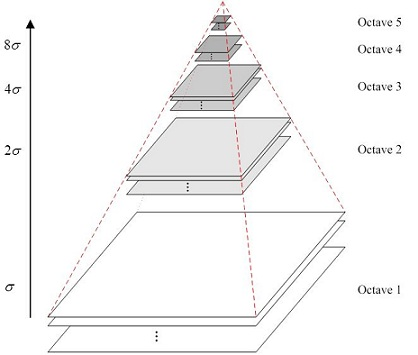
\includegraphics{gausspy}
\caption{图像的一组高斯金字塔}
\label{fig:gausspy}
\end{figure}

高斯金字塔是尺度空间的表示,sift算法是基于尺度空间理论的。尺度空间思想最早是由Iijima\upcite{Iijima}于1962年提出的,后经witkin\upcite{Witkin}和Koenderink\upcite{Koenderink}等人的推广逐渐得到关注,在计算机视觉邻域使用广泛。尺度空间理论的基本思想是:在图像信息处理模型中引入一个被视为尺度的参数,通过连续变化尺度参数获得多尺度下的尺度空间表示序列,对这些序列进行尺度空间主轮廓的提取,并以该主轮廓作为一种特征向量,实现边缘、角点检测和不同分辨率上的特征提取等。尺度理论的数学表达式如公式~\ref{chidu}所示:
\begin{equation}\label{chidu}
L(x,y,\delta)=G(x,y,\delta)*I(x,y)
\end{equation}

其中,*表示卷积运算,G(x,y,$\delta$)为高斯函数,
\begin{equation}\label{gauss}
G(x,y,\delta)=\frac{1}{2\pi{\delta}^2}e^{-\frac{(x-m/2)^2+(y-n/2)^2}{2\delta^2}}
\end{equation}

其中,m和n表示高斯模板的维度,(x,y)代表图像的像素位置,$\delta$是尺度空间因子,值越小表示图像被平滑的越少,相应的尺度也就越小。大尺度对应于图像的概貌特征,小尺度对应于图像的细节特征。

\item 高斯差分金字塔建立\\高斯差分金子塔是在高斯金子塔的基础上的到得,通过将同一组中的相邻层数的高斯图像相减,可以得到高斯差分图像,具体如图~\ref{fig:gaussDog}所示:
\begin{figure}[htp]
\centering
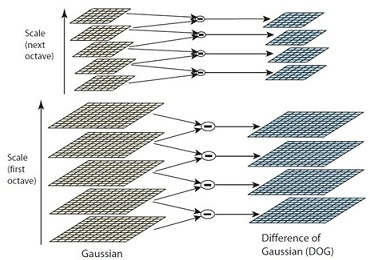
\includegraphics{gaussDog}
\caption{高斯差分金子塔}
\label{fig:gaussDog}
\end{figure}

尺度归一化的高斯拉普拉斯函数${\delta}^2{\nabla}^2{G}$的极大值和极小值同其它的特征提取函数,例如:梯度,Hessian或Harris角特征比较,能够产生最稳定的图像特征。而高斯差分函数(Difference of Gaussian ,简称DOG算子)与尺度归一化的高斯拉普拉斯函数${\delta}^2{\nabla}^2{G}$,它们的关系推导如下:
\begin{equation}\label{dog_1}
\frac{\partial{x}}{\partial{\delta}}=\delta\nabla^2G
\end{equation}

利用差分近似代替微分,则有:
\begin{equation}\label{dog_2}
\delta\nabla^2G=\frac{\partial{x}}{\partial{\delta}}\approx\frac{G(x,y,k\delta)-G(x,y,\delta)}{k\delta-\delta}
\end{equation}

因此就有:
\begin{equation}\label{dog_3}
G(x,y,k\delta)-G(x,y,\delta)\approx(k-1)\delta^2\nabla^2G
\end{equation}

其中k-1是常数,并不影响极值点的位置求取,两者极值关系如图~\ref{fig:py_dog}所示,其中横坐标为0处,最下方的曲线为高斯差分算子,上方为高斯拉普拉斯算子:
\begin{figure}[htp]
\centering
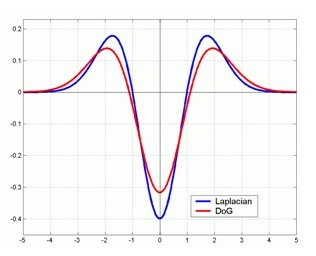
\includegraphics{py_dog}
\caption{高斯拉普拉斯和高斯差分极值关系对比}
\label{fig:py_dog}
\end{figure}

当使用高斯差分算子代替拉普拉斯算子进行极值检测,公式如下所示:
\begin{equation}\label{dog_detect}
D(x,y,\delta)=\Bigl(G(x,y,k\delta)-G(x,y,\delta)\Bigr)*I(x,y)=L(x,y,k\delta)-L(x,y,\delta)
\end{equation}

在实际计算时,使用高斯金字塔每组中相邻上下两层图像相减,得到高斯差分图像,然后在差分图像上进行极点检测。
\item 极点检测\\关键点是由DOG空间的局部极值点组成的,关键点的初步探查是通过同一组内各DoG相邻两层图像之间比较完成的。为了寻找DoG函数的极值点,每一个像素点要和它所有的相邻点比较,看其是否比它的图像域和尺度域的相邻点大或者小。如图3.4所示,中间的检测点和它同尺度的8个相邻点和上下相邻尺度对应的9×2个点共26个点比较,以确保在尺度空间和二维图像空间都检测到极值点。具体如图~\ref{fig:pole_detect}所示:
\begin{figure}[htp]
\centering
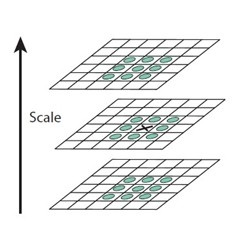
\includegraphics{pole_detect}
\caption{高斯差分图像上的极点检测}
\label{fig:pole_detect}
\end{figure}

\item 关键点精确定位\\离散空间的极值点并不是真正的极值点,图~\ref{fig:keypoint_detect}显示了二维函数离散空间得到的极值点与连续空间极值点的差别。利用已知的离散空间点插值得到的连续空间极值点的方法叫做子像素插值(Sub-pixel Interpolation)。
\begin{figure}[htp]
\centering
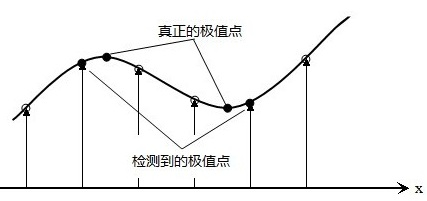
\includegraphics{keypoint_detect}
\caption{离散空间与连续空间极值点的差别}
\label{fig:keypoint_detect}
\end{figure}

为了提高关键点的稳定性,需要对尺度空间DoG函数进行曲线拟合。利用DoG函数在尺度空间的Taylor展开式(拟合函数)如公式~\ref{Tayor},其中$X={(x,y,\delta)^T}$代表相对插值中心的偏移量,当它在任一维度上的偏移量大于0.5时(即x或y或$\delta$),意味着插值中心已经偏移到它的邻近点上,所以必须改变当前关键点的位置,同时在新的位置上反复插值直到收敛,但是此过程有可能超出设定测迭代次数或者图像边界范围,那么这样的点就应该被删除掉,在Lowe的论文中,迭代的上限为5。另外,${|D(x)|}$的值过小会受到噪声影响而变得不稳定,因此该值小于某个阈值的极值点也要删除,在Lowe论文中,使用阈值的大小为0.03。
\begin{equation}\label{Tayor}
D(X)=D+\frac{\partial{D}^T}{\partial{X}}X+\frac{1}{2}X^T\frac{\partial^2{D}}{\partial{X}^2}X
\end{equation}

\item 关键点方向分配和描述\\为了使描述符具有旋转不变性,需要利用图像的局部特征为给每一个关键点分配一个基准方向。使用图像梯度的方法求取局部结构的稳定方向。对于在DOG金字塔中检测出的关键点点,采集其所在高斯金字塔图像3σ邻域窗口内像素的梯度和方向分布特征。梯度的模值和方向如下:
\begin{equation}\label{mozhi}
m(x,y)=\sqrt{L(x+1,y)-{L(x-1,y)}^2+L(x,y+1)-{L(x,y-1)}^2}
\end{equation}
\begin{equation}\label{fangxiang}
\theta(x,y)=\tan^{-1}\Bigl({\frac{L(x,y+1)-L(x,y-1)}{L(x+1,y-L(x-1,y)}}\Bigr)
\end{equation}
\end{compactenum}

其中,L为关键点所在尺度的空间值,邻域窗口半径为3*1.5${\delta}$。

在完成关键点的梯度计算后,使用直方图统计邻域内像素的梯度和方向。梯度直方图将0~360度的方向范围分为36个柱(bins),其中每柱10度。如图~\ref{fig:direct_histogram}所示,直方图的峰值方向代表了关键点的主方向,(为简化,图中只画了八个方向的直方图)。方向直方图的峰值则代表了该特征点处邻域梯度的方向,以直方图中最大值作为该关键点的主方向。为了增强匹配的鲁棒性,只保留峰值大于主方向峰值80%的方向作为该关键点的辅方向。因此,对于同一梯度值的多个峰值的关键点位置,在相同位置和尺度将会有多个关键点被创建但方向不同。仅有15%的关键点被赋予多个方向,但可以明显的提高关键点匹配的稳定性。
\begin{figure}[htp]
\centering
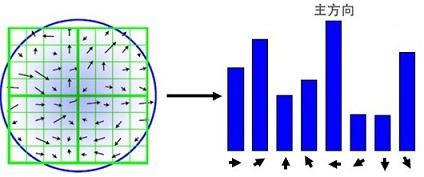
\includegraphics{direct_histogram}
\caption{关键点方向直方图}
\label{fig:direct_histogram}
\end{figure}

在关键点方向被确定之后,我们需要给这些关键点建立一个定量的描述,该描述子不仅包括关键点的信息,也包含关键点周围对其有贡献的像素点,并且描述符应该有较高的独特性,以便于提高特征点正确匹配的概率。SIFT算法中通过一组向量将关键点的特征描述出来,SIFT描述子是关键点邻域高斯图像梯度统计结果的一种表示。通过对关键点周围图像区域分块,计算块内梯度直方图,生成具有独特性的向量,这个向量是该区域图像信息的一种抽象,具有唯一性。

Lowe在论文中建议使用在关键点尺度空间内4*4的窗口中计算的8个方向的梯度信息,共4*4*8=128维向量表征,具体表示步骤如下:
\begin{itemize}
\item 确定计算描述子所需的图像区域
\item 将坐标轴旋转为关键点的方向,以确保旋转不变性
\item 将邻域内的采样点分配到对应的子区域内,将子区域内的梯度值分配到8个方向上,计算其权值
\item 插值计算每个种子点八个方向的梯度
\item 描述子向量门限
\item 按特征点的尺度对特征描述向量进行排序
\end{itemize}

至此,SIFT特征描述向量生成完毕。

在上述5个步骤中,构建高斯金字塔和极点检测是最为耗时的两个。构建高斯金字塔时需要对每张图片进行高斯滤波,高斯滤波是一个时间复杂度为O(N3) 的操作,这里的N与图像大小成正比。图~\ref{fig:gausspy}中仅显示了一组金字塔,而SIFT算法往往需要构建多组金字塔,使得构建高斯金字塔的时间复杂度达到O(O*I*N3),其中O为高斯塔的组数,I为高斯塔的层数。极点检测则是在整个金字塔组上进行的,相当于在一个维度为4的空间(组,层,长,宽)中搜索极值点,它的时间复杂度为O(O*I*N2)。SIFT算法流程中既包含高斯滤波和图像缩放等通用性较强的操作,也含有构建高斯(查分)金字塔、极点检测、消除边缘响应等通用性较差的操作。它的空间复杂度和时间复杂度都比较高,当有海量的图片需要进行特征提取时,占用内存较多,所需的处理时间也会很长。这也是我们使用Spark去加速SIFT算法的原因。

只有充分理解SIFT算法原理之后,才能比较好的在Spark上实现大规模特征提取工作。

\section{Spark核心技术原理}
在这一小节中,将会对Spark中三个核心技术原理进行分析,它们分别是内存编程原理,任务调度原理,性能优化。这三个技术在本文的设计起非常重要的地位,只有将这些技术理解透彻后,才能自如的解决开发过程中遇到的问题。
\subsection{Spark内存编程原理}
Spark区别于其他的大数据处理框架,比如Hadoop\upcite{Hadoop},在于它是一个内存计算的大数据处理框架,它可以将处理的中间结果保存在内存中,后续的计算可以在此基础上直接运行,提升了执行的效率。那么,这么多的数据保存在内存中,这就必须基于分布式内存的数据结构抽象,让开发人员基于该数据结构进行操作,只要操作这些数据,它们就是位于集群的内存中的。上面说的内存抽象数据结构就是RDD(Resilient Distributed Dataset弹性分布式数据集),RDD是Spark最核心的概念,接下来将从RDD的底层实现原理,RDD的操作类型,RDD的缓存原理,RDD 的依赖关系和DAG的生成这几方面分析RDD。
\subsubsection{RDD的底层实现原理}
RDD的基本单元是分区(Partition),一个RDD由多个分区组成,每个分区都会被逻辑映射成一个Block,一个Block会被一个Task执行,这些Block由BlockManager管理,BlockManager负责管理这些Block在集群内的分布。整个过程如图~\ref{fig:blockmanager}所示:
\begin{figure}[htp]
\centering
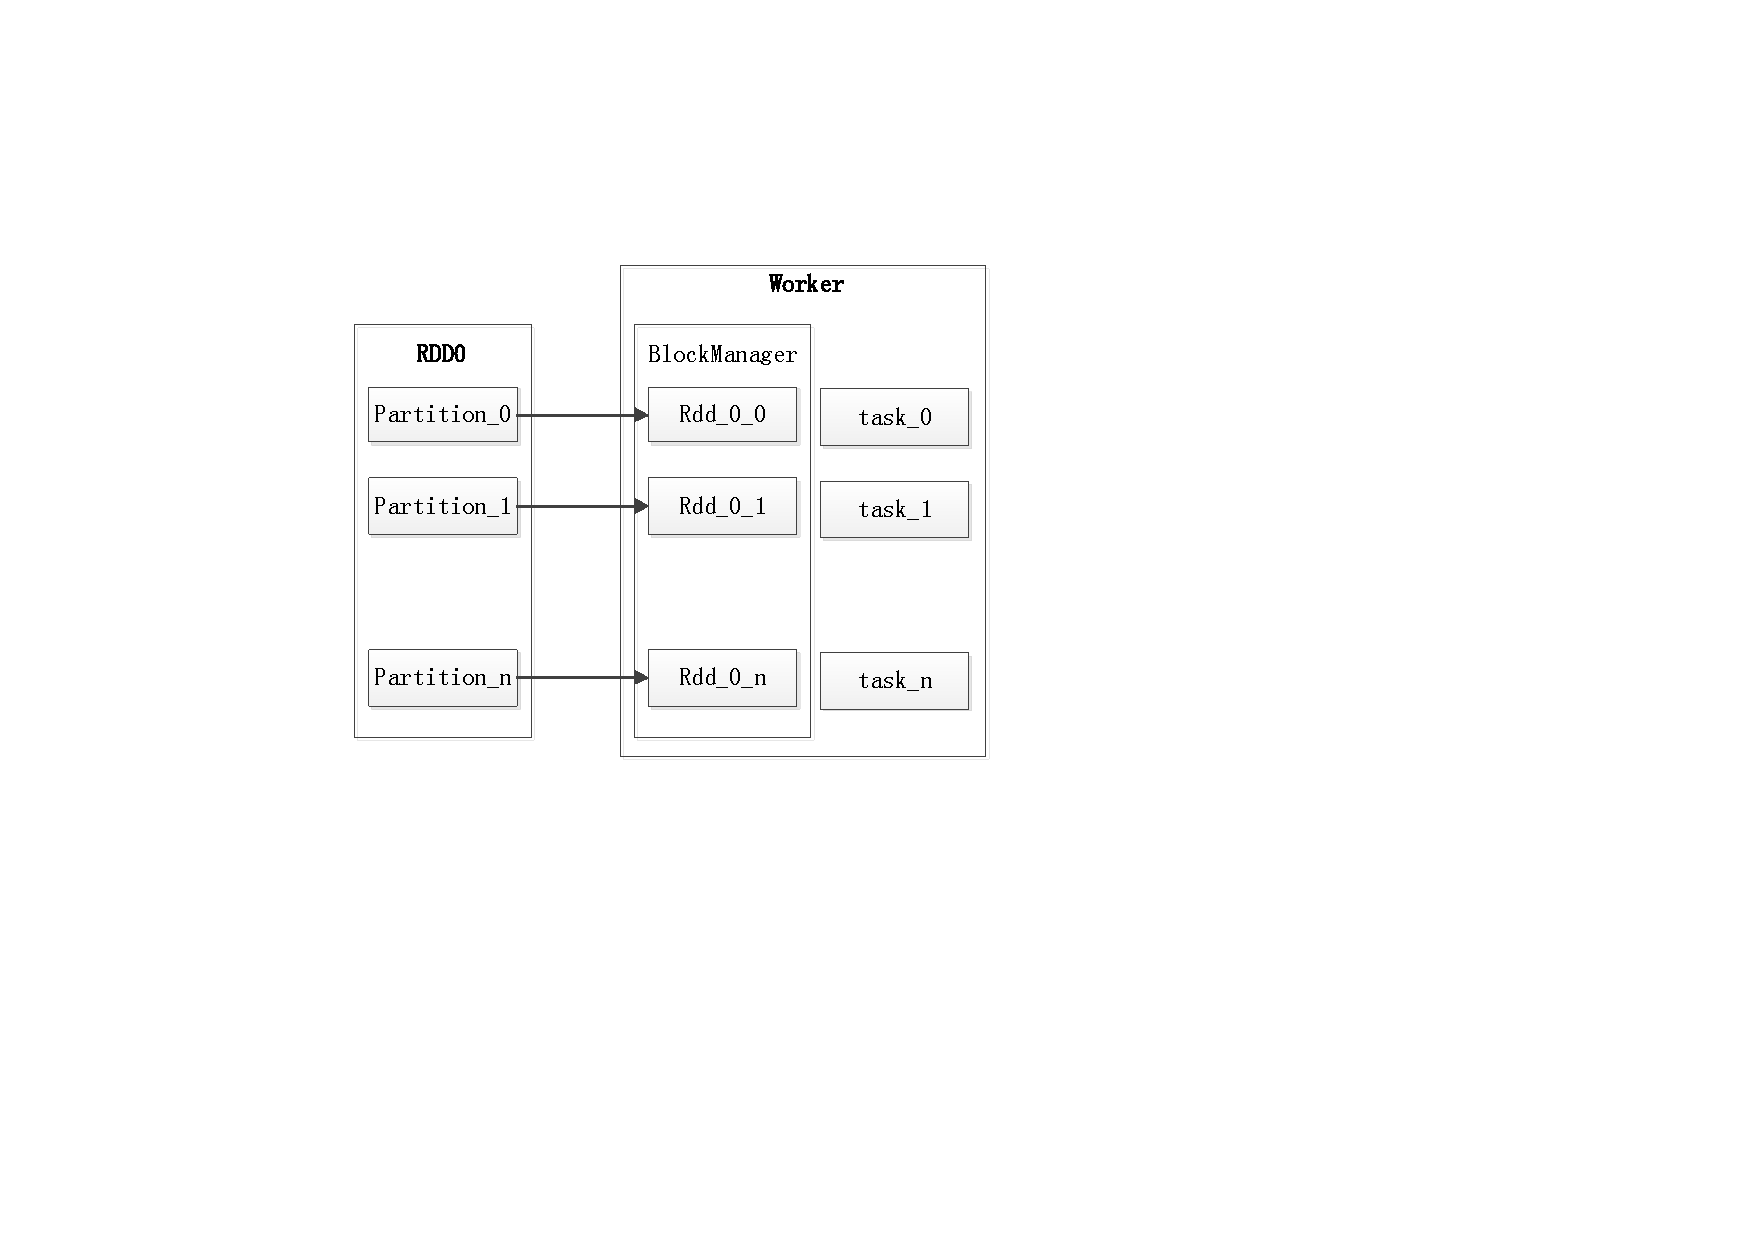
\includegraphics{blockmanager}
\caption{RDD Partition的存储和计算模型}
\label{fig:blockmanager}
\end{figure}

\subsubsection{RDD的操作类型}
RDD提供的操作可以分为两种类型,分别是transformtion(转换)和action(动作),表\ref{tab:trans}和表\ref{tab:action}分别列出了常用的转换操作和动作操作。所有的转换操作都是惰性的,被调用时,它们不会直接计算结果,它们只是记住上一个转换动作,当一个动作操作被调用时,这些转换操作才会被执行。这种设计会让Spark运行得更加高效率,因为可能在动作操作时,被操作的数据集会变得比较小。
\begin{table}[h] %开始一个表格environment,表格的位置是h,here。
\caption{RDD转换操作} %显示表格的标题
\centering
\label{tab:trans}
\begin{tabular}{p{6cm}|p{8cm}} %设置了每一列的宽度,强制转换。
\hline
\hline
转换  & 含义 \\ %用&来分隔单元格的内容 \\表示进入下一行
\hline %画一个横线,下面的就都是一样了,这里一共有4行内容
map(func)  & 返回一个新的分布式的数据集,该数据集有每一个输入元素经过func函数转换后组成\\
\hline
filter(func)  & 返回一个新的数据集,该数据集经过func函数计算后返回值为true的输入元素组成\\
\hline
flatMap(func)  & 类似于Map,但是每一个输入元素可以被映射为0个或者是多个输出元素\\
\hline
mapPartitions(func) & 类型于map,但是独立在RDD的每一个分片上运行,因此func的类型必须是Iterator[T]=>Iterator[U]\\
\hline
mapPartitionWithSplit(func) & 类似于mapPartitions,但是func带有一个整型参数表示分片的索引值,func的函数类型为(Int,Iterator[T])=>Iterator[U]\\
\hline
sample(withReplacement,fraction,seed) & 根据fraction指定比例对数据进行采用\\
\hline
union(otherDataset) & 返回一个新的数据集,新数据集是由源数据集和参数数据集联合而成的\\
\hline
distinct(numTasks) & 返回一个包含源数据集中所有不重复的元素的新的数据集\\
\hline
\hline
\end{tabular}
\end{table}

\begin{table}[h] %开始一个表格environment,表格的位置是h,here。
\caption{RDD动作操作} %显示表格的标题
\centering
\label{tab:action}
\begin{tabular}{p{6cm}|p{8cm}} %设置了每一列的宽度,强制转换。
\hline
\hline
动作  & 含义 \\ %用&来分隔单元格的内容 \\表示进入下一行
\hline %画一个横线,下面的就都是一样了,这里一共有4行内容
reduce(func)  & 通过函数func聚集数据集中的所有元素\\
\hline
collect()  & 在驱动程序中,以数组的形式返回数据集中的所有元素。通常在使用filter或者其他操作返回一个足够小的数据子集后再使用比较有用\\
\hline
count()  & 返回数据集的个数\\
\hline
first() & 返回数据集的第一个元素\\
\hline
take(n) & 返回一个由数据集的前n个元素组成的数组\\
\hline
takeSample(withReplacement,num,seed) & 返回一个数组,该数组由从数据集中随机采用的num个元素组成\\
\hline
saveAsTextFile(path) & 将数据集的元素以textFile的形式保存到本地文件系统,HDFS或者任何Hadoop支持的文件系统\\
\hline
saveAsSequenceFile(path) & 将数据集的元素以Hadoop sequencefile的格式保存到指定目录下,可以是本地系统,HDFS或者任何Hadoop支持的文件系统\\
\hline
countByKey() & 对(K,V)类型的RDD有效,返回一个(K,Int)对的map,表示每一个key的元素个数\\
\hline
foreach(func) & 在数据集的每一个元素上,运行函数func进行更新\\
\hline
\hline
\end{tabular}
\end{table}

\subsubsection{RDD的缓存原理}
spark速度非常快的原因之一,就是在不同操作中内存中持久化(或缓存)一个数据集。当持久化一个RDD后,每一个节点都将会把计算分片的结果保存在内存中,后续的其他操作可以直接使用该结果,这就使得后续的动作变得十分迅速。

通过persist()或cache()方法可以标识一个要被持久化的RDD,一旦首次被触发后,该RDD将会被保留在计算节点的内存中并重用。persist()和cache()的实现如下:
\begin{lstlisting}[language=Java,numbers=none,frame=none]
/**Persist this RDD with the default storage level('MEMORY_ONLY').*/
def persist(): this.type = persist(StorageLevel.MEMORY_ONLY)
/**Persist this RDD with the default storage level('MEMORY_ONLY').*/
def cache(): this.type = persist()
\end{lstlisting}

假设首先进行了RDD0$\rightarrow$RDD1$\rightarrow$RDD2的计算作业,如果RDD1已经被缓存在内存中,那么后续在进行RDD0$\rightarrow$RDD1$\rightarrow$RDD3的计算作业时,就不需要从头开始,直接从RDD1往下执行作业即可,因此计算速度得到了很大的提升,具体过程如下图\ref{fig:rdd_cache}所示:
\begin{figure}[htp]
\centering
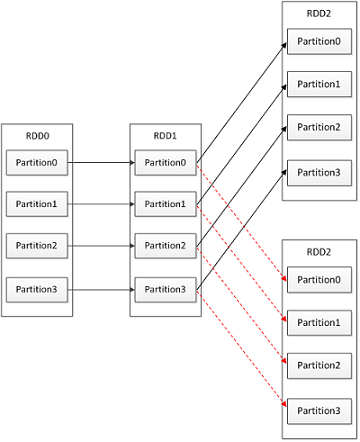
\includegraphics{rdd_cache}
\caption{RDD 缓存加速原理}
\label{fig:rdd_cache}
\end{figure}

缓存的rdd有可能会丢失,或者因为内存不足而删除,但是rdd有完整的容错机制,保证在rdd丢失或者删除的情况下计算依然可以正确执行。
\subsubsection{RDD的依赖关系和DAG的生成}
一个Spark应用中,不同的RDD间存在依赖关系,依赖关系分为窄依赖(narrow dependency)和宽依赖(wide dependency),窄依赖和宽依赖的定义如下:
\begin{itemize}
\item 窄依赖,窄依赖是指父RDD的每个分区只被子RDD的一个分区所使用,如图\ref{fig:dependency}左边部分显示
\item 宽依赖,宽依赖是指父RDD的每个分区都可能被多个子RDD分区所使用,如图\ref{fig:dependency}右边部分显示
\end{itemize}
\begin{figure}[htp]
\centering
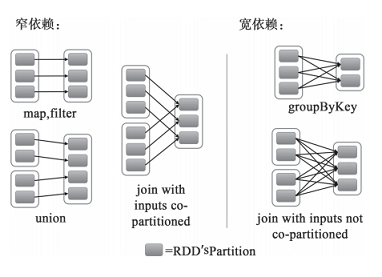
\includegraphics{dependency}
\caption{RDD窄依赖和宽依赖对比}
\label{fig:dependency}
\end{figure}
在Spark应用开发中,RDD会经过很多转换操作,每个转换操作都会生成一个新的RDD,这些转换操作最后会形成一个有向图(Directed Acyclic Graph,简称DAG)。这个DAG记录着RDD间的依赖关系,借助这些依赖关系,能保证一个RDD被计算前,所有它所依赖的parent RDD都已经完成了计算。同时Spark 也是整个DAG根据依赖关系的不同划分为不同的阶段(stage),一个stage中包含的一组并行执行的任务。划分stage的依据是,rdd间是窄依赖关系的划分到一个stage中,rdd间是宽依赖的划分到不同的stage中。一个stage中可以并行执行,不同stage 间顺行执行。
\subsection{Spark任务调度原理}
Spark任务调度框架主要由三个模块支撑起,它们分别是DAGScheduler,SchedulerBackend及TaskScheduler。首先DAGScheduler分析用户提交的应用,根据依赖关系建立DAG,然后将DAG 划分为不同的Stage,而stage中包含所要执行的tasks。SchedulerBackend负责整个集群交互,收集可用的资源信息,然后将这些信息上报TaskScheduler。TaskScheduler将从SchedulerBackend获取到的资源信息以及从DAGScheduler生成的tasks进行一个资源的分配,将tasks分配的合适的资源上面。整个流程如图\ref{fig:schedulerfw}所示:
\begin{figure}[htp]
\centering
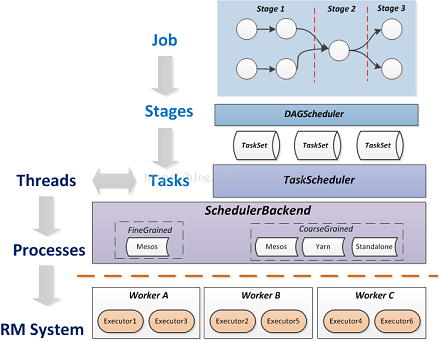
\includegraphics{schedulerfw}
\caption{Spark任务调度框架}
\label{fig:schedulerfw}
\end{figure}
\subsubsection{DAGScheduler}
DAGScheduler面向stage的调度(stage-oriented scheduling)的高级调度器,将job根据类型划分为不同的stage(划分的依据是依赖关系为窄依赖的属于一个stage,依赖关系为宽依赖的RDD属于不同的stage)为每个job 的不同stage 计算DAG,跟踪哪些RDD和stage被物化并且发现运行job的最小的调度策略,然后并在每一个stage 内产生一系列的task 并封装为taskset, 结合当前的缓存情况来决定每个Task的最佳位置(任务在数据所在的节点上运行),以taskset 为单位提交(submitTasks) 给TaskScheduler。
\subsubsection{SchedulerBackend}
SchedulerBackend负责与Cluster Manager交互,取得该Application分配到的资源,并且将这些资源传给TaskScheduler,由TaskScheduler为Task最终分配计算资源。在不同的集群模式下,SchedulerBackend的实现是不一样的,实现可以分为细粒度和粗粒度两种。分为细粒度和粗粒度两种。细粒度只有Mesos(mesos有粗细两种粒度的使用方式)实现了,粗粒度的实现者有yarn,mesos,standalone。拿standalone模式来说粗粒度,每台物理机器是一个worker,worker一共可以使用多少cpu和内存,启动时候可以指定每个worker起几个executor,即进程,每个executor的cpu和内存是多少。粗粒度与细粒度的主要区别,就是粗粒度是进程long-running 的,计算线程可以调到executor上跑,但executor的cpu和内存更容易浪费。细粒度的话,可以存在复用,可以实现抢占等等更加苛刻但促进资源利用率的事情。这俩概念还是AMPLab论文里最先提出来并在Mesos里实现的。AMPLab在资源使用粒度甚至任务分配最优的这块领域有不少论文,包括Mesos的DRF算法、Sparrow调度器等。所以standalone模式下,根据RDD的partition数,以及每个task需要的cpu 数,可以很容易计算每台物理机器的负载量、资源的消耗情况、甚至知道TaskSet要分几批才能跑完一个stage。
\subsubsection{TaskScheduler}
TaskScheduler负责Application的不同Job间的调度,在Task执行失败时启动重试机制。TaskScheduler里会对已经提交的tasks进行一次优先级排序,这个排序策略目前有两种:FIFO(First In First Out,先进先出)或FAIR(公平调度),默认调度策略是FIFO。通过排序,会得到一份待运行的tasks,然后就把从schedulerBackend交过来的worker资源信息合理分配给这些tasks。分配前,为了避免每次都是前几个worker被分到tasks,所以先对WorkerOffer列表进行一次随机洗牌。接下来就是遍历tasks,看workers的资源“够不够”,“符不符合”task,如果符合的话task就被正式launch起来。
\subsection{Spark性能优化原理}
在本小节中,将介绍Spark的性能优化原理,因为Spark是处理大数据的框架,因此性能优化是非常有必要的。接下来将从几个方面分析spark的性能问题
\subsubsection{调度和分区优化}
在spark应用程序中,会经常使用fiter算子进行数据过滤,而频繁的过滤或者过滤的数据量过大就会造成大量小分区,由于spark是每个数据分区都会分配一个任务执行,如果任务过多,就会造成线程切换开销很大,很多任务等待执行,并行度实际上不高。面对这种情况,我们可以采用RDD中的重分区函数进行数据的紧缩,减少分区数,将小分区合并成大分区。具体可以通过coalesce函数进行,函数定义如下:
\begin{lstlisting}[language=Java,numbers=none,frame=none]
def coalesce(numPartitions: Int, shuffle: Boolean = false)(implicit ord: Ordering[T] = null): RDD[T]
\end{lstlisting}

该函数会返回一个含有numPartitions数量个分区的新的RDD,即将整个RDD重分区。

使用这个函数会出现一个问题,比如将1000个分区的RDD重分区为一个分区,就会造成数据过于集中,完成无法开掘集群并行计算的能力。在这种情况下,可以将coalsesce 函数参数shuffle 设置为true,由于shuffle 可以分隔shuffle,这就保证了上游的任务仍是1000个,否则两个上下游的任务合并为一个stage 计算,这个stage就会在一个分区上进行并行计算。

除了将分区收缩,在某些情况下,可能会对原来的分区进行扩充,将分区数量增加,以利用并行计算能力。在这个过程中,默认使用的是Hash分区器进行重分区。

在分区优化问题中,还有一个倾斜(skew)的问题。倾斜是一个大数据处理中一个非常重要的问题,可以分为数据倾斜和任务倾斜,数据倾斜的结果就会造成任务倾斜,在个别分区上,任务的执行时间过长。
\begin{compactenum}
\item 数据倾斜\\产生数据倾斜的原因大致有这几种:
\begin{itemize}
\item key数据分布不均匀,因为spark中默认是按照Hash方式进行分区,如果某个key的数据特别多,就会造成分到某个key上的数据特别多,最后造成某个分区的数据特别多,也就出现了数据倾斜。
\item 结构化数据表设计问题
\item 某些SQL语句产生数据倾斜
\end{itemize}

\item 任务倾斜\\产生任务倾斜的原因较为隐蔽,有可能是服务器架构的原因,有可能是JVM的原因,有可能是线程池的原因,也有可能是业务本省的原因。比如在本文设计中就发现,即使是两个任务的处理数据的总大小一样,但是仍然会产生任务倾斜,这和处理问题的具体场景有关系,在SIFT算法中,算法的时间复杂度和图片的尺寸大小有关系的。
\end{compactenum}

\subsubsection{内存存储优化}
因为spark是内存计算的大数据处理框架,因此内存存储优化也是十分重要的内容。内存调优过程中,有三个方向值得考虑,分别是JVM调优,OOM问题调优及磁盘临时目录空间优化。
\begin{compactenum}
\item JVM调优\\不同的JAVA对象都有一个对象头,这些信息有时候比数据本身的信息还要大,比如只有一个Int属性的对象。还有一些链式结构,它们会包含一些指针信息。因此在开发的过程要选好数据类型和数据结构,尽量减少一些链式结构的使用;减少对象的嵌套;可以考虑使用数字ID或者是枚举对象,而不是字符串作为key的关键数据。
\item OMM问题调优\\在spark开发过程中,内存溢出(OutOfMemoryError)是一个经常会遇到的问题,发生内存溢出的原因是Java虚拟机创建的对象太多,在进行垃圾回收时,虚拟机分配的堆空间已经用满了,与heap space有关。解决这类问题有两种思路,一种是减少App的内存占用空间消耗,另一种是增大内存资源的供应。具体设计时,可以查看程序中是否有循环创建对象的地方,程序中应该减少这种代码的存在,或者可以调整JVM中的Xmx(最大堆)和Xms(最小堆)参数的大小。另外,还要查看在做shuffle类操作符时是否创建的Hash表过大,在这种情况下,可以通过增加任务数,即分区数来提升并行度,减少每个任务的输入数据,减少内存占用来解决问题。
\end{compactenum}

\subsubsection{磁盘临时目录空间优化}
Spark在进行shuffle的过程中,中间结果会写到spark在磁盘的临时目录中,如果临时目录过小的话,会造成No Space left on device异常,在这种情况下可以配置多个盘块来扩展Spark的磁盘临时目录,让更多的数据可以写到磁盘,加快I/O速度。
\subsubsection{网络传输优化}
Spark是大数据处理框架,因此集群中数据传输也是影响应用性能的重要因素。如果可以减少数据传输的次数或者是传输的大小,可能会极大的提高应用的性能。下面将分析spark中数据传输优化的场景。
\begin{compactenum}
\item 大局部变量的传输\\默认情况下,算子函数内,如果使用了外部变量,那么会将这个变量的拷贝到执行这个函数的每一个task中,如果这个变量十分大,比如是一个大数组,而且执行的任务又特别多,那么网络的传输耗费就会特别大。下面就是一个例子的展示,其中factor就是一个变量,它在map任务中被使用:
\begin{lstlisting}[language=Java,numbers=none,frame=none]
val factor = 3
rdd.map(num => num*factor)
\end{lstlisting}

面对这种情况,可以使用Spark的Brodcast(广播)变量对数据传输进行优化,通过Brocast变量将用到的大数据量数据进行广播发送,可以提升整体速度。Broadcast主广播的变量是只读的,并且在每个节点上只会有一份副本,而不会为每个task都拷贝一个副本。因此就减少了变量到各个节点的网络传输消耗,以及在各个节点上的内存消耗。
\item 大结果收集\\在spark的开发中,会经常用到collect操作,collect操作将各个分区的结果收集到一个数组,返回到driver。如图\ref{fig:collect}如果收集的结果过大,就会拖慢应用的执行时间,甚至造成内存溢出。
\begin{figure}[htp]
\centering
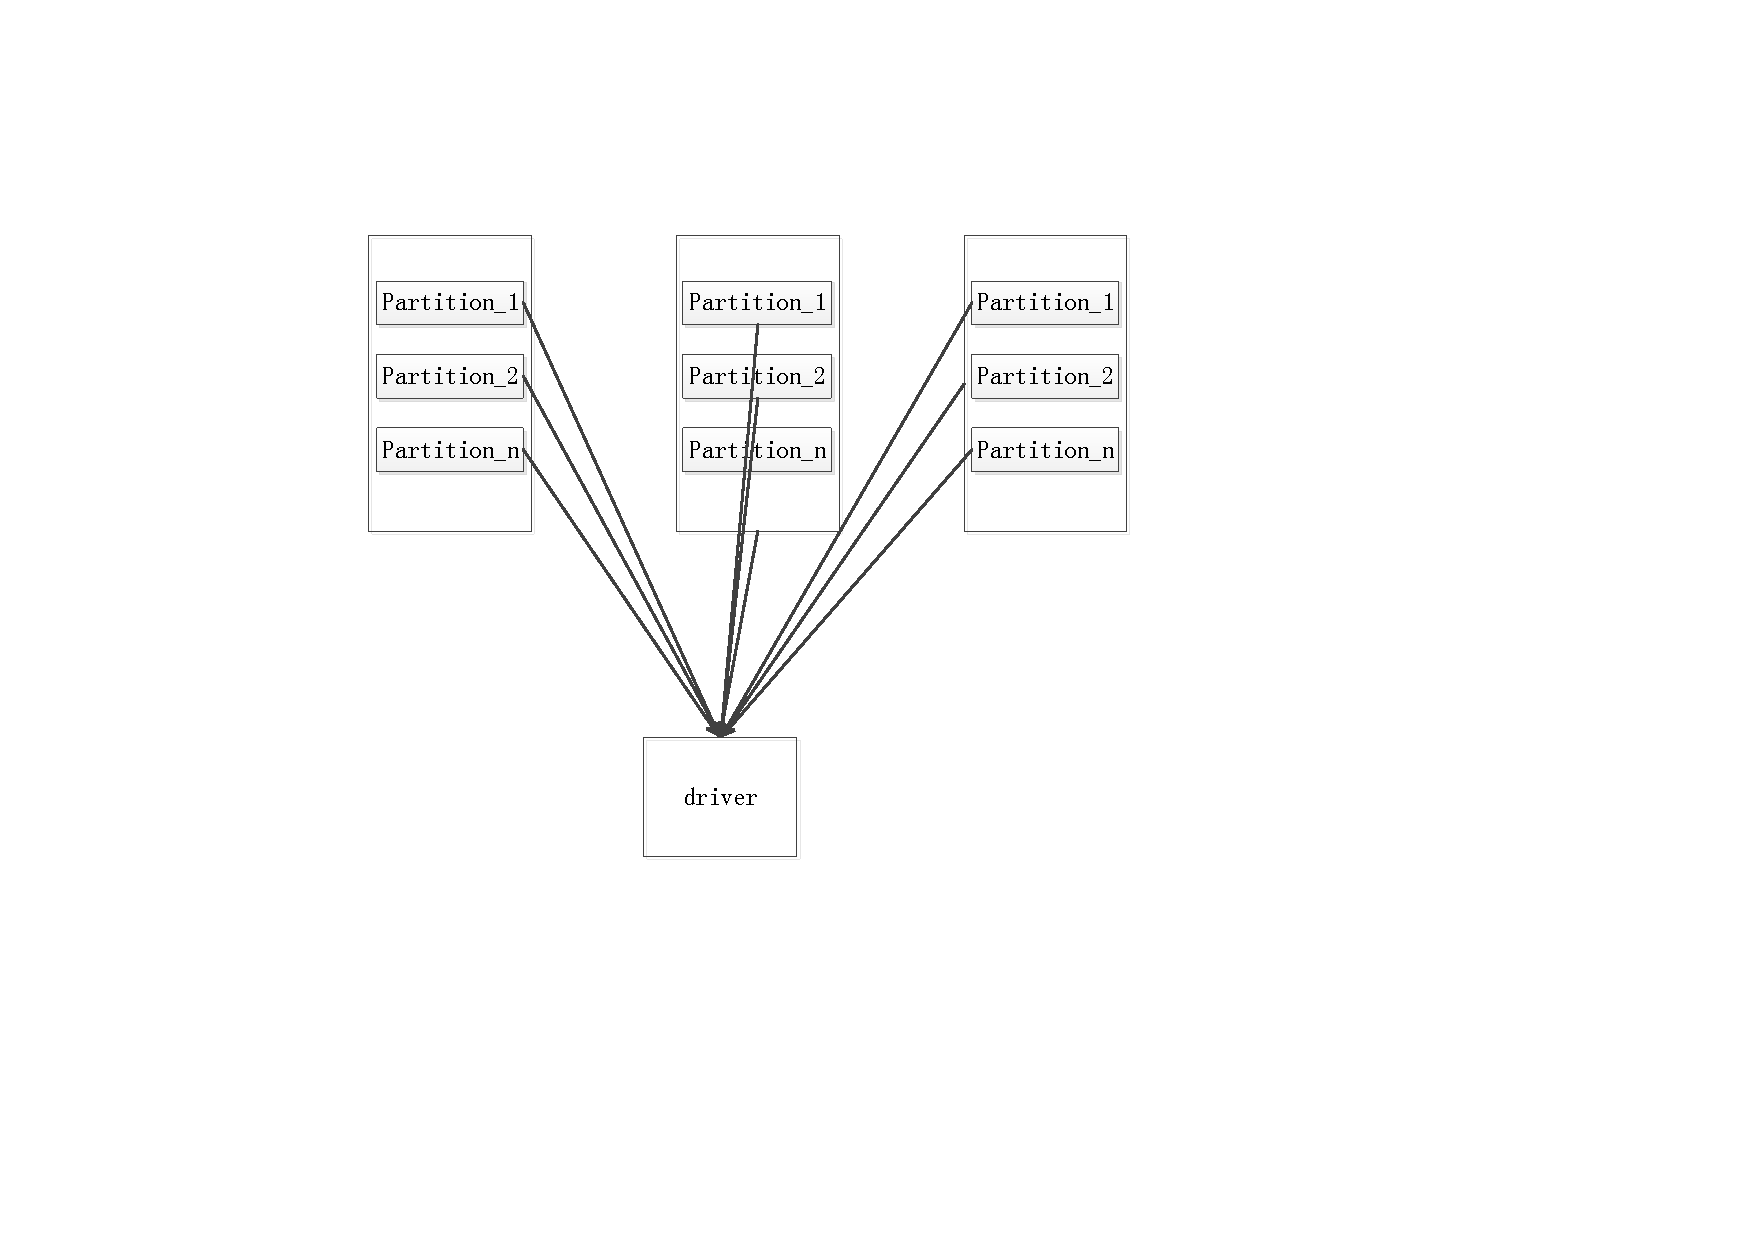
\includegraphics{collect}
\caption{collect操作收集所有分区}
\label{fig:collect}
\end{figure}
面对这种情况,如果收集的结果过大,可以将数据分布式的存储在HDFS或者其他的分布式持久化层上,这样可以减少单机数据的I/O开销和单机内存的存储压力。
%%\subsubsection{序列化与压缩}
\end{compactenum}
\section{分布式存储原理}

\section{GPU特征提取原理}

\section{本章小结}
本章分析了本文工作的一些技术原理,首先分析SIFT算法原理,主要针对SIFT算法的5个主要步骤进行分析,分析其数学原理及作用,然后讨论了算法的时间复杂性。接着介绍了作为本文设计的计算引擎Spark,主要涉及了Spark核心技术原理,主要包括Spark的内存编程原理,任务调度原理,性能优化原理。最后介绍了本文设计中作为存储层的分布式文件系统HDFS的一些核心原理。最后,介绍了作为本文设计的比较的GPU特征提取原理。





%%% Local Variables:
%%% mode: latex
%%% TeX-master: "../main"
%%% End:

\begin{ack}
在论文完成之际,我想对在我求学路上帮助过我,引导过我,关心过我的父母,老师,同学和朋友们致以由衷的感谢! 

感谢我的导师沈立老师,沈老师在我的研究生阶段给了我很大的帮助。刚进入研究生时候,研究生和本科学习上的差异是使得我感到迷茫,沈老师在这时候帮我规划好科研方向,制定好目标,使得我逐渐的适应研究生的生活和学习。之后,沈老师不断的带领我们进行科研攻关,教会我们如何发现问题,怎样去思考问题,在组会上,沈老师总是能抓住问题的要害,分析出问题的根本,在沈老师的带领下,我的科研能力不断提高,逐渐体会到科研的快乐。进入课题之后,沈老师不断的和我讨论课题的方向,帮助我制定好课题的方向,之后沈老师严格的监督我课题的进展,耐心的指导我解决课题中的难题,在沈老师的帮助下,我的课题按照预定目标顺利完成。整个研究生阶段,我在沈老师的悉心指导下,综合素质得到了很大的提高,所以再次向沈老师表示衷心的感谢!

感谢于齐师兄,于齐师兄在我进入实验室后,一直都给予我帮助。于齐师兄为人厚道,热心帮助别人,在我遇到困难的时候,师兄总是向我伸出援手,帮助我解决问题。感谢同队的张万新师兄,万新师兄在我的硕士课题上给予我很大的帮助,在我遇到困惑时,师兄总是不厌其烦的给我讲解,直到我的困惑被彻底解决。感谢钱程师兄,王博千师兄,王璐师姐,徐叶茂师兄,李宁师兄,陈静玮师姐,感谢你们对我的帮助和关怀!

感谢同级同学的刘文杰,番丝江,何锡明,和你们在一起的日子里,我过得十分开心,你们的存在使得我的研究生生涯充满了欢乐!感谢李临同学,和你一块参加比赛,战斗的日子里,我留下了许多美好的回忆!

感谢张诗琴师妹,杨耀华师弟,感谢你们对我课题上的帮助!

感谢我的父母,他们在我常长的路上付出了无比的艰辛,父母用他们辛勤的劳作换来了我现在安逸的生活。感谢我的伯父,他在人生路上给予了我很大帮助,伯父坚韧的性格一直是我学习的榜样。感谢我的大姐,大姐在我成长的路上给了我很大的帮助,无论是在学习上,工作上还是生活上,姐姐总是不断的鼓励我,帮助我,关怀我。家人,你们无条件的爱是我强大的后盾!

最后,感谢在预审,评阅及答辩过程中对我论文提出宝贵意见的给我专家与老师!
\end{ack}


%</thesis>
%    \end{macrocode}
%
% 在\LaTeX{}下管理参考文献将极其方便,建议使用Jabref生成条目,
% 用\verb|\cite|(其中\verb|upcite|是上标索引)索引即可。
% \verb|refs.bib|是你的参考文献名。
%    \begin{macrocode}
%<*thesis>
\cleardoublepage
\phantomsection
\addcontentsline{toc}{chapter}{参考文献}
\bibliographystyle{bstutf8}
\bibliography{ref/refs}

\begin{resume}

  \section*{发表的学术论文} % 发表的和录用的合在一起

  \begin{enumerate}[{[}1{]}]
  \addtolength{\itemsep}{-.36\baselineskip}%缩小条目之间的间距,下面类似
  \item Zhang xinming, Yang yaohua, Shen Li, Spark-SIFT:A Spark-Based Large-Scala Image Feature Extract System, SKG2017.
  \end{enumerate}

  \section*{学科竞赛成果} % 有就写,没有就删除
  \begin{enumerate}[{[}1{]}]
  \addtolength{\itemsep}{-.36\baselineskip}%
  \item 2017华为软件精英挑战赛武长赛区一等奖;
  \item 2016三一重工校园APP设计大赛冠军;
  \item 2016华为软件精英挑战赛武长赛区二等奖;
  \end{enumerate}
\end{resume}

%</thesis>
%    \end{macrocode}
%
%<thesis>% 最后,需要的话还要生成附录,全文随之结束。
%    \begin{macrocode}
%<*thesis>
\appendix
\backmatter
% TeX
\chapter{模板提供的希腊字母命令列表}

大写希腊字母:
\begin{table}[htbp]
\centering
\begin{tabular}{llll}
\toprule
$\Gamma$~\verb|\Gamma| & $\Lambda$~\verb|\Lambda| & $\Sigma$~\verb|\Sigma| & $\Psi$~\verb|\Psi| \\
$\Delta$~\verb|\Delta| & $\Xi$~\verb|\Xi| & $\Upsilon$~\verb|\Upsilon| & $\Omega$~\verb|\Omega| \\
$\Theta$~\verb|\Theta| & $\Pi$~\verb|\Pi| & $\Phi$~\verb|\Phi| & \\
\midrule
$\varGamma$~\verb|\varGamma| & $\varLambda$~\verb|\varLambda| & $\varSigma$~\verb|\varSigma| & $\varPsi$~\verb|\varPsi| \\
$\varDelta$~\verb|\varDelta| & $\varXi$~\verb|\varXi| & $\varUpsilon$~\verb|\varUpsilon| & $\varOmega$~\verb|\varOmega| \\
$\varTheta$~\verb|\varTheta| & $\varPi$~\verb|\varPi| & $\varPhi$~\verb|\varPhi| & \\
\bottomrule
\end{tabular}
\end{table}

小写希腊字母:
\begin{table}[htbp]
\centering
\begin{tabular}{llll}
\toprule
$\alpha$~\verb|\alpha| & $\theta$~\verb|\theta| & $o$~\verb|o| & $\tau$~\verb|\tau| \\ 
$\beta$~\verb|\beta| & $\vartheta$~\verb|\vartheta| & $\pi$~\verb|\pi| & $\upsilon$~\verb|\upsilon| \\ 
$\gamma$~\verb|\gamma| & $\iota$~\verb|\iota| & $\varpi$~\verb|\varpi| & $\phi$~\verb|\phi| \\ 
$\delta$~\verb|\delta| & $\kappa$~\verb|\kappa| & $\rho$~\verb|\rho| & $\varphi$~\verb|\varphi| \\ 
$\epsilon$~\verb|\epsilon| & $\lambda$~\verb|\lambda| & $\varrho$~\verb|\varrho| & $\chi$~\verb|\chi| \\ 
$\varepsilon$~\verb|\varepsilon| & $\mu$~\verb|\mu| & $\sigma$~\verb|\sigma| & $\psi$~\verb|\psi| \\ 
$\zeta$~\verb|\zeta| & $\nu$~\verb|\nu| & $\varsigma$~\verb|\varsigma| & $\omega$~\verb|\omega| \\ 
$\eta$~\verb|\eta| & $\xi$~\verb|\xi| & $\varkappa$~\verb|\varkappa| & $\digamma$~\verb|\digamma| \\ 
\midrule
$\upalpha$~\verb|\upalpha| & $\uptheta$~\verb|\uptheta| & $\mathrm{o}$~\verb|\mathrm{o}| & $\uptau$~\verb|\uptau| \\ 
$\upbeta$~\verb|\upbeta| & $\upvartheta$~\verb|\upvartheta| & $\uppi$~\verb|\uppi| & $\upupsilon$~\verb|\upupsilon| \\ 
$\upgamma$~\verb|\upgamma| & $\upiota$~\verb|\upiota| & $\upvarpi$~\verb|\upvarpi| & $\upphi$~\verb|\upphi| \\ 
$\updelta$~\verb|\updelta| & $\upkappa$~\verb|\upkappa| & $\uprho$~\verb|\uprho| & $\upvarphi$~\verb|\upvarphi| \\ 
$\upepsilon$~\verb|\upepsilon| & $\uplambda$~\verb|\uplambda| & $\upvarrho$~\verb|\upvarrho| & $\upchi$~\verb|\upchi| \\ 
$\upvarepsilon$~\verb|\upvarepsilon| & $\upmu$~\verb|\upmu| & $\upsigma$~\verb|\upsigma| & $\uppsi$~\verb|\uppsi| \\ 
$\upzeta$~\verb|\upzeta| & $\upnu$~\verb|\upnu| & $\upvarsigma$~\verb|\upvarsigma| & $\upomega$~\verb|\upomega| \\ 
$\upeta$~\verb|\upeta| & $\upxi$~\verb|\upxi| & & \\ 
\bottomrule
\end{tabular}
\end{table}

希腊字母属于数学符号类别,请用\verb|\bm|命令加粗,其余向量、矩阵可用\verb|\mathbf|。


\end{document}
%</thesis>
%    \end{macrocode}
%
% 当然还有一些收尾工作,校验审阅自不必说。接下来你需要:修改论文中英文日期,
% 生成盲评,生成明(盲)评A3封面。
%
% {\color{blue}Happy \TeX{}ing! 欢迎提各式各样的意见!}
%
% \newpage\relax%
%
% \StopEventually{\PrintChanges}
% \clearpage
%
% \section{实现细节}
% 我们首先介绍文档模板的基本信息以及宏包和配置,
% 然后依照国防科学技术大学论文模板的书写规范一节一节的介绍实现步骤。
%
% \changes{v1.2}{2009/09/28}{添加了A3封面制作}
%
% \subsection{基本信息}
%    \begin{macrocode}
%<cls>\NeedsTeXFormat{LaTeX2e}[1999/12/01]
%<cls>\ProvidesClass{nudtpaper}
%<cfg>\ProvidesFile{nudtpaper.cfg}
%<cls|cfg>[2011/07/17 v2.2 NUDT paper template]
%    \end{macrocode}
%
% \subsection{宏包配置}
%
%<*cls>
%
%\changes{v0.99}{2009/08/17}{add package options}
% 当前的宏包选项在之前已经介绍了,下面是实现步骤,就是几个\verb|if|。
%\changes{v1.6}{2009/12/01}{添加单独的单双面控制}
%\changes{v2.0}{2010/11/09}{添加盲评控制}
%
%    \begin{macrocode}
\newif\ifismaster\ismastertrue
\DeclareOption{master}{\ismastertrue}
\DeclareOption{doctor}{\ismasterfalse}
\newif\ifisanon\isanonfalse
\DeclareOption{anon}{\isanontrue}
\newif\ifistwoside\istwosidefalse
\DeclareOption{twoside}{\istwosidetrue}
\DeclareOption*{\PackageWarning{nudtpaper}{Unknown Option '\CurrentOption'}}
% handle fonts
\newif\ifisttf\isttffalse
\newif\ifisotf\isotffalse
\newif\ifisfz\isfzfalse
\newif\ifisfandol\isfandolfalse
\DeclareOption{ttf}{\isttftrue}
\DeclareOption{otf}{\isotftrue}
\DeclareOption{fz}{\isfztrue}
\DeclareOption{fandol}{\isfandoltrue}
\ProcessOptions\relax
%    \end{macrocode}
%
% 首先调用在文档类书写中需要的过程控制语句,在计算一些\verb|length|时要用到
%    \begin{macrocode}
\RequirePackage{ifthen,calc}
%    \end{macrocode}
%
% 接着我们导入文本类,该模板基于标准的书籍模板book,其默认格式为单面打印。
% 博士论文如需双面打印,必须指定\verb|twoside|选项。双开的含义是章节总是
% 起在右手边,左手空白页为完全的空白页,不包含页眉页脚。
%
% \changes{v1.6}{2009/12/01}{修改开关选项}
%
%    \begin{macrocode}
\ifistwoside
  \LoadClass[a4paper,12pt,openright,twoside]{book}
\else
  \LoadClass[a4paper,12pt,openany]{book}
\fi
%    \end{macrocode}
%
% 我们直接用\textsf{geometry}宏包进行页面边距的设定,调用titlesec设定标题以及页眉页脚,
% 用\textsf{titletoc}设定目录格式。需要改动的可以参考这三个宏包的说明文档。
%
%    \begin{macrocode}
\RequirePackage[includeheadfoot]{geometry}
\RequirePackage[center,pagestyles]{titlesec}
\RequirePackage{titletoc}
%    \end{macrocode}
%
% 文档中另外重要的两个部分是表格和图片。
% 首先来看图片:\textsf{graphicx}宏包是必不可少的,
% 并排图形。\textsf{subfigure} 已经不再推荐,用新的 \textsf{subfig}。
% 加入 \verb|config| 选项
% 以便兼容 \textsf{subfigure} 的命令。浮动图形和表格标题样式。\textsf{caption2} 已经不
% 推荐使用,采用新的 \textsf{caption}。它会自动被 \textsf{subfig} 装载进来。所以可以在
% 后面使用 \textbf{captionsetup} 命令,宏包\textsf{float}的作用是可以用H命令,
% 将浮动对象强制放在这里(副作用是版面可能不好):
%
%    \begin{macrocode}
\RequirePackage{graphicx}
\RequirePackage[config]{subfig}
\RequirePackage{float}
%    \end{macrocode}
%
% 再来看表格:我们采用\textsf{longtable}来处理长的表格,还需要\textsf{array}包;
% 标准的论文需要表格为三线表,这里引用\textsf{booktabs}宏包来处理,
% 这样,我们就可以简单的使用\verb|\toprule|,\verb|\midrule|,\verb|bottomrulle|
% 这样的命令;
% 为了在表格中支持跨行,需要引入\textsf{multirow}包,\textsf{tabularx}的作用是为了使用
% 固定宽度的表格,\textsf{slashbox}可以让我们在表格中使用反斜线:
%    \begin{macrocode}
\RequirePackage{array}
\RequirePackage{longtable}
\RequirePackage{booktabs}
\RequirePackage{multirow}
\RequirePackage{tabularx}
\RequirePackage{slashbox}
%    \end{macrocode}
% 表格和图片的例子可以搜索C\TeX{}论坛或者看示例文件。
%
% 引入\textsf{paralist}来达到比较好看的列表环境
%    \begin{macrocode}
\RequirePackage[neverdecrease]{paralist}
%    \end{macrocode}
%
% 文档中还需要一定的色彩控制和字体控制
%    \begin{macrocode}
\RequirePackage{xcolor}
%    \end{macrocode}
%
% 为了排出漂亮的数学公式,\textsf{amsmath}包是必不可少的,
% 需要注意的是,新版本的论文模不再使用\textsf{txfonts}宏包,
% 为了支持希腊正体字母,需要调用\verb|upgreek.sty|,使用方法是\verb|\up<greek>|。
% 注意到这个宏包前面加上了\verb|Symbolsmallscale|选项,这是为了调整希腊字母的大小而设定的。
% 如果用户不满意这个宏包的积分号
% 等符号,倾向与使用传统的\LaTeX{}风格的数学符号,那么可以使用
% \textsf{mathptmx}宏包,但要把\verb|upgreek|的选项改为\verb|Symbol|,要不然
% 正体希腊字母要显得比正常字符小一点哦。
% 而大写斜体希腊字母(变量)可以通过\textsf{amsmath}的\verb|\var<Greek>|得到。
% 对于希腊字母的加粗使用\verb|bm|宏包,而一般变量的加粗那就使用\verb|\mathbf|吧!
% \changes{v2.0}{2010/11/09}{去掉fontspec,传递no-math到xeCJK,加入bm宏包}
% \changes{v2.2}{2011/07/16}{去掉txfonts宏包,使用lm字体,添加svgreek.sty}
% \changes{v2.2}{2011/07/16}{修改,仍旧使用upgreek, mathptmx, bm组合}
% \changes{v2.2}{2011/09/25}{修改,使用upgreek, txfonts, bm组合}
% \changes{v2.2}{2012/11/28}{给用户提供额外的选项,还是mtpro比较漂亮}
% \changes{v2.3}{2013/12/27}{调整数学字体,加入mtpro使用说明,并且仿照IEEE模板,修改displaypenalty}
% \changes{v2.5}{2015/05/11}{去掉txfonts,用默认数学字体}
%    \begin{macrocode}
\RequirePackage{amsmath,amssymb}
\RequirePackage[Symbolsmallscale]{upgreek}
%\RequirePackage{amsmath}
%\RequirePackage[amsbb,eufrak,compatiblegreek,subscriptcorrection,nofontinfo]{mtpro2}
\interdisplaylinepenalty=2500
\RequirePackage{bm}
\RequirePackage[T1]{fontenc}
\RequirePackage[amsmath,thmmarks,hyperref]{ntheorem}
%    \end{macrocode}
% 需要注意的是,如果用户有\verb|mtpro2|包,还是强烈建议使用这个的,因为数学公式
% 在这个包下显得特别的美观。虽然下载和安装不属于这篇使用说明的范畴,但是,上面的注释部分
% 可以给大家如何使用的一个简单的例子。当你安装好\verb|mtpro2|之后,主要取消注释,并且将
% 上面的三个包注释掉即可。
%
% 本文档类直接采用\XeTeX{}引擎,方便了字体配置以及编译,
% 这里需要调用\textsf{XeCJK}宏包,no--math的作用是不改变先前数学宏包设定的数学字体。
% 同时采用\textsf{indentfirst}宏包管理文字的缩进:
% \changes{v1.8}{2010/10/15}{修改了默认的xeCJK的选项,为了兼容旧的xeCJK版本,normalindentfirst选项暂不使用,而是在后面添加indentfirst包}
% \changes{v2.0}{2010/11/10}{传递no-math给xeCJK里面的fontspec宏包}
% \changes{v2.2}{2011/07/03}{移除CJKtextspace, CJKmathspace, CJKnumber选项}
% \changes{v2.4}{2015/02/09}{移除CJKnumber选项,添加新的CJKnum宏包。旧版本TexLive无需更改。}
%
%    \begin{macrocode}
\RequirePackage[CJKchecksingle,no-math]{xeCJK}
\RequirePackage{CJKnumb}
\RequirePackage{indentfirst}
%    \end{macrocode}
%
% 另外一个关键部分是文献索引,包括书签以及参考文献的索引,记得\textsf{hyperref}配合
% \XeTeX{}使用时暂不能开启Unicode选项,新的发行版已经移除\textsf{hypernat}包。
% 另外还要注意,你最终的打印版肯定不希望有花花绿绿的链接对吧?
% 那就把下面那行\verb|hyperref|注释掉就行了或者把选项改为\verb|\colorlinks=false|即可。
% \changes{v2.1}{2010/12/29}{移除hypernat包}
% \changes{v2.2}{2011/07/17}{移除hyperref的CJKbookmarks旋向}
% \changes{v2.3}{2013/12/27}{加入色彩版hyperref}
% \changes{v2.5}{2015/05/11}{提示用户在最终打印版时去掉链接颜色}
%    \begin{macrocode}
\RequirePackage[numbers,sort&compress,square]{natbib}
\RequirePackage[colorlinks=true,linkcolor=blue,citecolor=red,pdfborder=0 1 1]{hyperref}
%\RequirePackage[pdfborder=0 0 1]{hyperref}
%    \end{macrocode}
%</cls>
%
%\subsection{基础配置}
% 本章主要介绍模板中用到的基本的元素和定义,现在包括两部分: 字体,字号和字体命令
%
%\subsubsection{字体定义}
% 我们首先来处理\TeX{}中最令人棘手的字体问题,
% 在使用\textsf{XeCJK}包之后,配置和选择很容易,
% 预先设定好一些字体命令是为了后面方便的更改文本字体的需要。
% 首先我们开启\TeX{}连字符:
%    \begin{macrocode}
%<*cls>
\defaultfontfeatures{Mapping=tex-text}
%</cls>
%    \end{macrocode}
%
% 之后用\textsc{XeCJK}包提供的命令设定字体,用户可以选择使用TTF还是OTF字体,
% Adobe的OpenType字体在排版上更具备优势,文档显示锐利,推荐使用。
% 另外在这一个新版本中,我们推荐用户也可以使用方正的字体,只要使用\verb|FZ|选项即可。
% 中注释掉相关的字体就可以。方正字体的有点是标点符号的位置无需修正,且字体之间配合很好。
% \verb|setcharclass|的作用是纠正xunicode、xeCJK的一些设定:
%
% \changes{v0.99}{2009/08/17}{add options TTF and OTF}
% \changes{v1.9}{2010/10/28}{定义一个cusong字体,使用的是中宋}
% \changes{v2.3}{2013/12/27}{用户可以考虑使用方正字体,加入FZ选项}
% \changes{v2.5}{2015/05/11}{重新更改字体选项的调用方式,现在变成三个ttf、otf、fz}
% \changes{v2.5}{2015/05/11}{这种方式用户可以特别方便的添加自己的字体集}
%
%    \begin{macrocode}
%<*cls>
\xeCJKsetcharclass{"0}{"2E7F}{0}
\xeCJKsetcharclass{"2E80}{"FFFF}{1}

% ZhongYi 中易字体
\newcommand{\installttf}{
    %%%% Windows Thesis Fonts
    \setmainfont{Times New Roman PS Std}
    \setsansfont{Arial}
    \setmonofont{Courier New}
    %%%% Using Office Family Fonts
    \setCJKmainfont[BoldFont={STZhongsong}]{SimSun}
    \setCJKsansfont{SimHei} % Hei
    \setCJKmonofont{FangSong} % Fangsong 
    %%%% alias
    \setCJKfamilyfont{song}{SimSun}
    \setCJKfamilyfont{hei}{SimHei}
    \setCJKfamilyfont{fs}{FangSong} % fang-song
    \setCJKfamilyfont{kai}{KaiTi} % Kai
}

% Adobe 字体
\newcommand{\installotf}{
    %%%% Windows Thesis Fonts
    \setmainfont{Times New Roman PS Std}
    \setsansfont{Arial}
    \setmonofont{Courier New}
    %%%% Using Adobe Family Fonts
    \setCJKmainfont[BoldFont={STZhongsong}]{Adobe Song Std}
    \setCJKsansfont{Adobe Heiti Std} % Hei
    \setCJKmonofont{Adobe Fangsong Std} % Fangsong 
    %%%% alias
    \setCJKfamilyfont{song}{Adobe Song Std}
    \setCJKfamilyfont{hei}{Adobe Heiti Std}
    \setCJKfamilyfont{fs}{Adobe Fangsong Std} % fang-song
    \setCJKfamilyfont{kai}{Adobe Kaiti Std} % Kai
}

% fz 方正字体 [recommended]
\newcommand{\installfz}{
    %%%% Windows Thesis Fonts
    \setmainfont{Times New Roman PS Std}
    \setsansfont{Arial}
    \setmonofont{Courier New}
    %%%% Using Founder Family Fonts
    \setCJKmainfont[BoldFont={FZYaSong-DB-GBK}]{FZShuSong_GB18030-Z01}
    \setCJKsansfont{FZHei-B01} % Hei
    \setCJKmonofont{FZFangSong-Z02} % fs
    %%%% alias
    \setCJKfamilyfont{song}{FZShuSong_GB18030-Z01}
    \setCJKfamilyfont{hei}{FZHei-B01}
    \setCJKfamilyfont{fs}{FZFangSong-Z02} % fang-song
    \setCJKfamilyfont{kai}{FZKai-Z03} % Kai
}

% fandol [incomplete in 2015]
\newcommand{\installfandol}{
    %%%% Windows Thesis Fonts
    \setmainfont{Times New Roman PS Std}
    \setsansfont{Arial}
    \setmonofont{Courier New}
    %%%% Using Fandol Family Fonts
    \setCJKmainfont{FandolSong}
    \setCJKsansfont{FandolHei} % Hei
    \setCJKmonofont{FandolFang} % fs
    %%%% alias
    \setCJKfamilyfont{song}{FandolSong}
    \setCJKfamilyfont{hei}{FandolHei}
    \setCJKfamilyfont{fs}{FandolFang} % fang-song
    \setCJKfamilyfont{kai}{FandolKai} % Kai
}

\ifisttf
\installttf
\fi

\ifisotf
\installotf
\fi

\ifisfz
\installfz
\fi

\ifisfandol
\installfandol
\fi

%</cls>
%    \end{macrocode}
%
% \changes{v1.6}{2009/12/01}{替换OTF英文字体为标准Windows自带字体}
% \changes{v2.3}{2013/12/27}{添加FZ字体选项}
%
% 选定好字体之后,就是设定字体别名,这样我们就可以在文档的其他部分直接使用较短的命令来
% 指定特定的字体了:
%
%    \begin{macrocode}
%<*cls>
% command alias
\newcommand{\cusong}{\bfseries}
\newcommand{\song}{\CJKfamily{song}}     % 宋体
\newcommand{\fs}{\CJKfamily{fs}}         % 仿宋体
\newcommand{\kai}{\CJKfamily{kai}}       % 楷体
\newcommand{\hei}{\CJKfamily{hei}}       % 黑体
\def\songti{\song}
\def\fangsong{\fs}
\def\kaishu{\kai}
\def\heiti{\hei}
%</cls>
%    \end{macrocode}
%
% \subsubsection{字号定义}
%下面就是定义字号大小,这一部分我们有两个参考,其一是:
%
% \begin{verbatim}
% 参考科学出版社编写的《著译编辑手册》(1994年)
% 七号      5.25pt       1.845mm
% 六号      7.875pt      2.768mm
% 小五      9pt          3.163mm
% 五号      10.5pt       3.69mm
% 小四      12pt         4.2175mm
% 四号      13.75pt      4.83mm
% 三号      15.75pt      5.53mm
% 二号      21pt         7.38mm
% 一号      27.5pt       9.48mm
% 小初      36pt         12.65mm
% 初号      42pt         14.76mm
%
% 这里的 pt 对应的是 1/72.27 inch,也就是 TeX 中的标准 pt
% \end{verbatim}
%
% 另外一个来自WORD中的设定:
% \begin{verbatim}
% 初号 = 42bp = 14.82mm = 42.1575pt
% 小初 = 36bp = 12.70mm = 36.135 pt
% 一号 = 26bp = 9.17mm = 26.0975pt
% 小一 = 24bp = 8.47mm = 24.09pt
% 二号 = 22bp = 7.76mm = 22.0825pt
% 小二 = 18bp = 6.35mm = 18.0675pt
% 三号 = 16bp = 5.64mm = 16.06pt
% 小三 = 15bp = 5.29mm = 15.05625pt
% 四号 = 14bp = 4.94mm = 14.0525pt
% 小四 = 12bp = 4.23mm = 12.045pt
% 五号 = 10.5bp = 3.70mm = 10.59375pt
% 小五 = 9bp = 3.18mm = 9.03375pt
% 六号 = 7.5bp = 2.56mm
% 小六 = 6.5bp = 2.29mm
% 七号 = 5.5bp = 1.94mm
% 八号 = 5bp = 1.76mm
%
% 1bp = 72.27/72 pt
% \end{verbatim}
%
% 我们采用习惯的字号设定方法(也就是WORD中的设定),首先编写字体设置命令:
%
%\begin{macro}{\choosefont}
% 我们可以使用 |\choosefont| 来选择字体, 字体设定这些大多是从清华的模板拷过来的。
%
%    \begin{macrocode}
%<*cls>
\newlength\thu@linespace
\newcommand{\thu@choosefont}[2]{%
    \setlength{\thu@linespace}{#2*\real{#1}}%
    \fontsize{#2}{\thu@linespace}\selectfont}
\def\thu@define@fontsize#1#2{%
    \expandafter\newcommand\csname #1\endcsname[1][\baselinestretch]{%
    \thu@choosefont{##1}{#2}}}
%</cls>
%    \end{macrocode}
%\end{macro}
%
%设定具体的字体大小:
%
%    \begin{macrocode}
%<*cls>
\thu@define@fontsize{chuhao}{42bp}
\thu@define@fontsize{xiaochu}{36bp}
\thu@define@fontsize{yihao}{26bp}
\thu@define@fontsize{xiaoyi}{24bp}
\thu@define@fontsize{erhao}{22bp}
\thu@define@fontsize{xiaoer}{18bp}
\thu@define@fontsize{sanhao}{16bp}
\thu@define@fontsize{xiaosan}{15bp}
\thu@define@fontsize{sihao}{14bp}
\thu@define@fontsize{banxiaosi}{13bp}
\thu@define@fontsize{xiaosi}{12bp}
\thu@define@fontsize{dawu}{11bp}
\thu@define@fontsize{wuhao}{10.5bp}
\thu@define@fontsize{xiaowu}{9bp}
\thu@define@fontsize{liuhao}{7.5bp}
\thu@define@fontsize{xiaoliu}{6.5bp}
\thu@define@fontsize{qihao}{5.5bp}
\thu@define@fontsize{bahao}{5bp}
%</cls>
%    \end{macrocode}
%
%\subsubsection{自定命令}
% 有一些常量,测试,自定义的命令等都放在这里,待到论文逐渐完善之后再做定夺,
% 当然用户自己的命令也可以在此添加,事实上如果natbib传递的是superscript,
% \verb|cite|命令默认就成了上标了。这里不加入这个选项,而是单独编写一个命令:
%
%    \begin{macrocode}
%<*cls>
\newcommand{\upcite}[1]{\textsuperscript{\cite{#1}}} % 上标形式引用
\newcommand{\china}{中华人民共和国}
\def\nudtpaper{\textsc{Nudt}\textsc{Paper}}
\newcommand{\pozhehao}{\kern0.2em\rule[0.8ex]{1.6em}{0.1ex}\kern0.2em}
\newcommand{\xiaopozhe}{\kern0.2em\rule[0.8ex]{0.6em}{0.1ex}\kern0.2em}
%</cls>
%    \end{macrocode}
% \changes{v2.5}{2015/05/11}{添加了一个xiaopozhe命令,用作中文连词符}
%
%\subsubsection{中文元素}
%
% 默认的页面元素的英文名,诸如Contents为目录,Abstract为摘要等,
% 我们首先将他们一一中文化:
% \changes{v0.992}{2009/08/19}{修改图表编号格式}
% \changes{v1.3}{2009/10/14}{修改图目录和表目录}
%
%    \begin{macrocode}
%<*cls>
\renewcommand\contentsname{目\hspace{1em}录}
\renewcommand\listfigurename{图\hspace{1em}目\hspace{1em}录}
\renewcommand\listtablename{表\hspace{1em}目\hspace{1em}录}
\newcommand\listequationname{公式索引}
\newcommand\equationname{公式}
\renewcommand\bibname{参考文献}
\renewcommand\indexname{索引}
\renewcommand\figurename{图}
\renewcommand\tablename{表}
\renewcommand\appendixname{附录}
\def\CJK@today{\CJKdigits{\the\year} 年 \CJKnumber{\the\month} 月}
\newcommand\zhtoday{\CJK@today}
\newcommand\entoday{\today{}}
%</cls>
%    \end{macrocode}
%
% 好,下面就开始按照论文模板要求进行排版!
%
%\subsection{编写要求}
% 学校规定,论文需采用白色纸双面打印。
% 学位论文用A4($210mm\times{}297mm$)标准大小的白纸,
% 在打字或印刷时,要求纸的四周留足空白边缘,以便装订、复制和读者批注。
% 每一面的上方(天头)和下方(地角)分别留边25mm,左侧(订口)
% 和右侧(切口)分别留边30mm,页眉与页脚分别为23mm。
%
% 实现起来很简单,只要调用\textsf{geometry}的版面控制命令即可,
% 方法为先把word模板转化为PDF,
% 用Adobe的裁剪功能查看页边距,进行微调,直到比对正确为止,设定如下:
%
% \changes{v0.991}{2009/08/18}{modify bottom skip}
% \changes{v1.1}{2009/09/26}{修改footskip容限以及bottom的值,为了容下longtab的''下一页''}
% \changes{v1.4}{2009/10/28}{减小页眉skip 1mm,用word叠印}
% \changes{v1.4}{2009/10/30}{增大页眉sep .5mm,用word叠印}
%
%    \begin{macrocode}
%<*cls>
\geometry{top=21mm,bottom=25.5mm,left=30mm,right=30mm}
\geometry{headheight=9mm,headsep=1mm,footskip=9mm}
%</cls>
%    \end{macrocode}
%
%\subsection{页眉页脚}
%
% 我们采用titlesec进行页面配置。
% 页面中的主要元素有Chapter,Section,Subsection等元素的外观,
% 位置,颜色字体等,页面元素还包括页眉页脚。这种方法配置简便,易管理。
% 国防科大的论文需要在页眉处画两根横线,我们通过下面的命令实现:
%
%\begin{macro}{\setheadrule}
% 这个命令属于更改\textsf{titlesec}中的一个画页眉的命令,稍加调整:
% \changes{v0.991}{2009/08/18}{modify headrull, s.t. all geometry match}
% \changes{v1.9}{2010/10/28}{去掉headsep,修改headrule,在sethead后添加raisebox}
%
%    \begin{macrocode}
%<*cls>
\renewcommand\setheadrule[1]{%
  \ifdim#1=\z@
    \let\makeheadrule\@empty
  \else
    \def\makeheadrule{%
    \makebox[0pt][l]{\rule[.2\baselineskip]{\linewidth}{1.5pt}}%
    \rule{\linewidth}{1.5pt}}%
  \fi}
%</cls>
%    \end{macrocode}
%\end{macro}
%
% 由于Chapter第一页默认是\verb|plain|页面格式,
% 章节的其余部分是在Matter中设定的页面格式,为了简单起见,
% 我们就直接更改\verb|plain|页面设置,
% 要求为5号宋体居中放置,画页眉页脚,页脚为1磅黑线
%
% \changes{v0.992}{2009/08/20}{renewpagestyle里面前导的空格可能导致clearpage生成新的一页,将空格去掉}
% \changes{v0.993}{2009/08/26}{修改标题,博士硕士对应不同的页眉}
%
%    \begin{macrocode}
%<*cls>
\renewpagestyle{plain}{
\sethead{}{\raisebox{.65\baselineskip}{\songti \wuhao \ifisanon{~}\else{国防科学技术大学研究生院\@optionpaperclass{}学位论文}\fi}}{}%
\setfoot{}{{\songti \wuhao 第~\thepage~页}}{}%
\headrule%
\footrule%
}
\setfootrule{1bp}
%</cls>
%    \end{macrocode}
%
%\subsection{编写格式}
%
% 当页面设置好之后,就是在论文的不同部分分别调用,一般来说论文类的书籍
% 分为三个matter,为前言区(前置部分),正文区(主体),后文区(附录),
% 在国防科大论文书写要求中,
% 需要将摘要单独进行页码编号,其编号为小写罗马字母,为此,
% 可以将摘要单独设定为一个matter,
% 名叫就叫做MidMatter,称作摘要区。每个Matter我们都一一介绍。
%
% 首先看前置部分,主要包括封面,目录,摘要等,实现为:
%
%    \begin{macrocode}
%<*cls>
\renewcommand\frontmatter{%
    \if@openright\cleardoublepage\else\clearpage\fi
    \@mainmatterfalse
    \pagenumbering{Roman}
    \pagestyle{plain}}
\newcommand\midmatter{%
    \if@openright\cleardoublepage\else\clearpage\fi
    \@mainmatterfalse
    \pagenumbering{roman}
    \pagestyle{plain}}
%</cls>
%    \end{macrocode}
%
% 之后为文章的正文区,采用阿拉伯数字编页码:
%
%    \begin{macrocode}
%<*cls>
\renewcommand\mainmatter{%
    \if@openright\cleardoublepage\else\clearpage\fi
    \@mainmattertrue
    \pagenumbering{arabic}
    \pagestyle{plain}}
%</cls>
%    \end{macrocode}
%
% 最后是附录部分,由于他的章节标题与正文中不一样(不是第几章,而是附录几),
% 我们需要单独设定:
%
%    \begin{macrocode}
%<*cls>
\renewcommand\backmatter{%
    \if@openright\cleardoublepage\else\clearpage\fi
    \titleformat{\chapter}{\filcenter \heiti \sanhao}{附录\,\thechapter\,}{1em}{}
    \titlecontents{chapter}[0pt]{\vspace{0.25\baselineskip} \heiti \xiaosi[1.25]}
      {附录\,\thecontentslabel\quad}{}
      {\hspace{.5em}\titlerule*{.}\contentspage}
    \@mainmattertrue
    \pagestyle{plain}}
%</cls>
%    \end{macrocode}
%
% 我们重新定义\verb|cleardoublepage|,使得生成完全的空白页,页面模式为\verb|empty|
%    \begin{macrocode}
%<*cls>
\renewcommand\cleardoublepage{\clearpage\if@openright \ifodd\c@page\else
  \newpage{}
  \thispagestyle{empty}
  \vspace*{\fill}
  \begin{center}
  \end{center}
  \vspace*{\fill}
  \clearpage\fi\fi%
}
%</cls>
%    \end{macrocode}
%
%\subsubsection{前置目录}
% 前置部分的封面在后面详细介绍。首先看目录,要求为:
% 目次页由论文的章、节、条、项、附录等的序号、名称和页码组成,
% 另页排在序之后。目次页标注学位论文的前三级目录。
% 标题统一用“目录”,黑体3字号字居中,段前、段后间距为1行;
% 各章(一级目录)名称用黑体小4号字,段前间距为0.5行,
% 段后间距为0行; 其它(二、三级目录)用宋体小4号字,
% 段前、段后间距为0行。:
%
% 在\LaTeX{}中,Chapter在目录中默认是没有点的,我们加上,另外我们一并将
% 目录中的section和subsection设定好,
% \changes{v0.991}{2009/08/18}{modify TOC baselineskip and font lineskip to 1.25}
%
%    \begin{macrocode}
%<*cls>
\titlecontents{chapter}[0pt]{\vspace{0.25\baselineskip} \heiti \xiaosi[1.25]}
    {第\CJKnumber{\thecontentslabel}章\quad}{}
    {\hspace{.5em}\titlerule*{.}\contentspage}
\titlecontents{section}[2em]{\songti \xiaosi[1.25]}
    {\thecontentslabel\quad}{}
    {\hspace{.5em}\titlerule*{.}\contentspage}
\titlecontents{subsection}[4em]{\songti \xiaosi[1.25]}
    {\thecontentslabel\quad}{}
    {\hspace{.5em}\titlerule*{.}\contentspage}
%</cls>
%    \end{macrocode}
%
% 然后是表目录和图目录,内容用宋体小4号字,在同学使用模板时,需要标题对齐,
% 我们一并在这里实现:
% \changes{v0.993}{2009/08/25}{添加makebox使得图表标题对齐}
%
%    \begin{macrocode}
%<*cls>
\titlecontents{figure}[0pt]{\songti \xiaosi[1.25]}
    {\makebox[3.5em][l]{图~\thecontentslabel\quad}}{}
    {\hspace{.5em}\titlerule*{.}\contentspage}
\titlecontents{table}[0pt]{\songti \xiaosi[1.25]}
    {\makebox[3.5em][l]{表~\thecontentslabel\quad}}{}
    {\hspace{.5em}\titlerule*{.}\contentspage}
%</cls>
%    \end{macrocode}
%
% 书籍模板中,在LOF或者LOT章节之间会默认插入额外的距离,我们通过修改下面这个命令移除,
% 这个方法不是一个完美的办法,\textbf{注意}:下面的代码不要去深究或者理解,
% 这只是把book.cls中的内容复制过来,然后去掉包含addvspace命令的两行。
% 我实在找不出更加好的办法,如果你有,可以联系我。
%
% \changes{v0.993}{2009/08/25}{移除LOF及LOT中章节之间额外的距离}
%
%    \begin{macrocode}
%<*cls>
\renewcommand\chapter{\if@openright\cleardoublepage\else\clearpage\fi
                    \thispagestyle{plain}%
                    \global\@topnum\z@
                    \@afterindentfalse
                    \secdef\nudt@chapter\@schapter}
\def\nudt@chapter[#1]#2{
  \ifnum \c@secnumdepth >\m@ne
    \if@openright\cleardoublepage\else\clearpage\fi
    \phantomsection
    \if@mainmatter
      \refstepcounter{chapter}%
      \addcontentsline{toc}{chapter}%
        {\protect\numberline{\thechapter}#1}%
    \else
      \addcontentsline{toc}{chapter}{#1}%
    \fi
  \else
    \addcontentsline{toc}{chapter}{#1}%
  \fi
  \chaptermark{#1}%
  \if@twocolumn
    \@topnewpage[\@makechapterhead{#2}]%
  \else
    \@makechapterhead{#2}%
    \@afterheading
  \fi
}
%</cls>
%    \end{macrocode}
%
%\subsubsection{前置摘要}
%
% 摘要的要求为题目黑体3字号字居中,段前、段后间距为1行,内容用宋体小4号字,
% 英文摘要内容用Time New Roman小4号字。
% 中文关键字以黑体小4号字另起一行,排在摘要的下方,英文关键字用Arial小4号字。
%
% \changes{v1.8}{2010/10/15}{ABSTRACT和英文关键字需要用Arial字体}
% \changes{v2.5}{2015/05/11}{英文关键词也要加粗}
%    \begin{macrocode}
%<*cls>
\newcommand\cabstractname{摘\hspace{1em}要}
\newcommand\eabstractname{ABSTRACT}
\newcommand\ckeywordsname{关键词}
\newcommand\ckeywords[1]{{\hei\xiaosi \ckeywordsname: #1}}
\newcommand\ekeywordsname{Key Words}
\newcommand\ekeywords[1]{\textbf{\textsf{\xiaosi \ekeywordsname: #1}}}
\newenvironment{cabstract}{%
    \chapter{\cabstractname}
    \xiaosi
    \@afterheading}
    {\par\vspace{2em}\par}
\newenvironment{eabstract}{%
    \chapter{\textsf{\eabstractname}}
    \xiaosi
    \@afterheading}
    {\par\vspace{2em}\par}
%</cls>
%    \end{macrocode}
%
%\subsection{主体部分}
%
% \subsubsection{标题格式}
% 要求为:
% \begin{compactenum}
% \item	一级标题(章)用黑体3号字居中,1.25倍行距,段前、段后间距为1行,每一章从新的一页开始;
% \item	二级标题(节)用宋体4号粗体字居中,1.25倍行距,段前、段后间距为1行;
% \item	三级标题用黑体小4号字两端对齐,1.25倍行距,段前、段后间距为1行;
% \item	四级标题用宋体小4号粗体字两端对齐,1.25倍行距,段前间距为0.5行,段后间距为0行;
% \end{compactenum}
%
% \changes{v0.991}{2009/08/18}{按照要求设定标题}
% \changes{v0.992}{2009/08/19}{修改secnumdepth使得subsubsection可用}
% \changes{v1.1}{2009/09/26}{修改Title的spacing为弹性值}
% \changes{v1.2}{2009/10/06}{去掉弹性值,不去生成大量的空白}
% \changes{v1.4}{2009/10/28}{修改chapter段后行距为2ex,段前-1ex,保证上下对称}
% \changes{v1.4}{2009/10/29}{修改chapter段后行距为2.4ex,段前-1.2ex,保证上下对称}
%
% 当章节标题出现的新的一页时,会出现段前距过小的情况,按照milksea的说法是:
% 一般而言,当一个内容在一页开头时,前面的\verb|\vskip|不起作用;
% 类似地,一行开头\verb|\hskip|不起作用。这不是 BUG,如果需要总起效果的间距,
% 用\verb|\vspace*|,文档里面有这样的例子。参照titlesec的文档,需加上:
% \changes{v1.9}{2010/10/28}{增加sectionbreak,设定topskip为0pt}
%
%    \begin{macrocode}
%<*cls>
\newcommand{\sectionbreak}{%
\addpenalty{-300}%
\vspace*{0pt}%
}
\setlength{\topskip}{0pt}
%</cls>
%    \end{macrocode}
% \changes{v1.9}{2010/10/28}{在定义了粗宋字体之后,按照学位论文要求设定标题字体}
% \changes{v1.9}{2010/10/28}{使用了ttltips.pdf的设置chapter距顶端距离的办法}
% \changes{v2.3}{2013/12/27}{修改了footnotesize,当一页中有两个footnote时,间距调整正常}
% \changes{v2.3}{2013/12/27}{修改了titleformat和titlespacing的定制,更改英文字体,修正间距}
%
%    \begin{macrocode}
%<*cls>
\setcounter{secnumdepth}{3}
\setlength{\footnotesep}{2.2ex \@minus 2bp}
\titleformat{\chapter}{\filcenter\sf \heiti\sanhao[1.25]}{第\CJKnumber{\thechapter}章\,}{1em}{}
\titleformat{\section}{\filcenter\bfseries \cusong\sihao[1.25]}{\thesection}{1em}{}
\titleformat{\subsection}{\sf \heiti\xiaosi[1.25]}{\thesubsection}{1em}{}
\titleformat{\subsubsection}{\bfseries \cusong\xiaosi[1.25]}{\thesubsubsection}{1em}{}
\titlespacing{\chapter}{0pt}{2.4ex-\topskip-\heightof{A}}{2.4ex \@minus 2bp}
\titlespacing{\section}{0pt}{2ex-\heightof{a}}{2ex \@minus 2bp}
\titlespacing{\subsection}{2em}{2ex \@minus 2bp}{2ex \@minus 2bp}
\titlespacing{\subsubsection}{2em}{1ex \@minus 2bp}{1ex \@minus 2bp}
%</cls>
%    \end{macrocode}
%
% \changes{v2.5}{2015/05/11}{添加了subsubsection下1ex的距离}
%
%\subsubsection{正文字体}
% 首先确定正文中使用的字体,文档要求正文字体为小四,行距为固定值1.25倍,
% 中文字体为宋体,英文为{Times New Roman}
%
%\begin{macro}{\normalsize}
% 我们重新定义 |\normalsize| 来确定文档的正文字体,
% 同时修改正文中公式与文字间的距离:
% \changes{v1.9}{2010/10/28}{在normalsize后面每一行加上\%号来吃掉多余的空格}
% \changes{v2.2}{2011/07/16}{减小公式之间距离rubber space的上界}
% \changes{v2.2}{2011/09/25}{减小公式之间距离rubber space的下界}
% \changes{v2.3}{2013/12/27}{移除了abovedisplay的正向rubberspace}
%
%    \begin{macrocode}
%<*cls>
\renewcommand\normalsize{%
\@setfontsize\normalsize{12bp}{12.87bp}%
\renewcommand{\baselinestretch}{1.3}%
\setlength\abovedisplayskip{10bp \@minus 1bp}%
\setlength\abovedisplayshortskip{10bp \@minus 1bp}%
\setlength\belowdisplayskip{\abovedisplayskip}%
\setlength\belowdisplayshortskip{\abovedisplayshortskip}%
}
%</cls>
%    \end{macrocode}
%\end{macro}
%
% \changes{v0.991}{2009/08/18}{modify normalsize, which will cause headrule shift}
% \changes{v0.991}{2009/08/18}{add comment on displayskip}
% \changes{v1.0}{2009/09/22}{modify display skip}
%
%\subsubsection{正文段落}
% 接下来还有一个细节就是处理段落缩进,文档设定为首行缩进2个字符,
% 这一个命令需要在文档开始时自动执行:
%
% \changes{v1.3}{2009/10/03}{添加checkparameter这一选项,避免由于更新模板导致未定义的情况出现}
% \changes{v1.7}{2010/04/30}{应当在封面制作完后替换tabular}
% \changes{v2.5}{2015/05/12}{删除twochars囧}
%
%    \begin{macrocode}
%<*cls>
\newlength\CJK@twochars
\def\CJKindent{%
  \settowidth\CJK@twochars{中国}%
  \parindent\CJK@twochars}
\AtBeginDocument{%
  \CJKindent\relax
  \checkparameter\relax
}
%</cls>
%    \end{macrocode}
%
% 之后定义段落间距,段前间距以及段后间距都为0
% \changes{v0.993}{2009/08/27}{修改parskip}
% \changes{v2.2}{2011/09/25}{修改parskip,允许少量的调整,1bp}
% \changes{v2.2}{2011/10/14}{修改parskip,仅允许负的少量调整,2bp}
% \changes{v2.3}{2013/12/27}{移除parskip的正向rubberspace}
% \changes{v2.5}{2015/05/11}{减小parskip的负向距离至1bp}
%
%    \begin{macrocode}
%<*cls>
\setlength{\parskip}{0bp \@minus 1bp}
%</cls>
%    \end{macrocode}
%
% 有时候我们需要手动设定字体间距,该命令在声明页使用过:
%\begin{macro}{\ziju}
%    \begin{macrocode}
%<*cls>
\newcommand*{\ziju}[1]{\renewcommand{\CJKglue}{\hskip #1}}
%</cls>
%    \end{macrocode}
%\end{macro}
%
% \changes{v1.4}{2009/10/26}{推荐用户使用紧凑的列表环境}
%
% 这一部分来自Thuthesis的代码,其出发点是不满意\LaTeX{}默认列表环境间距过大,用
% paralist包中的相关环境进行替代。请参考paralist宏包。
%
% \changes{v1.4}{2009/10/26}{修改参考文献的行距设定}
%
% 而同样有间距问题的是参考文献,两个条目之间过大的距离不是很美观,
% 最简单的办法是修改bibsep变量,如果还是不行,我们直接从thuthesis中拿来代码:
%
% \changes{v1.4}{2009/10/26}{修改参考文献的行距}
% \changes{v1.4}{2009/10/29}{修改参考文献左对齐}
% \changes{v2.2}{2011/10/14}{减小文献列表间距,将penalty改为4000}
%
%    \begin{macrocode}
%<*cls>
\renewenvironment{thebibliography}[1]{%
   \chapter*{\bibname}%
   \list{\@biblabel{\@arabic\c@enumiv}}%
        {\renewcommand{\makelabel}[1]{##1\hfill}
         \settowidth\labelwidth{1.1cm}
         \setlength{\labelsep}{0.4em}
         \setlength{\itemindent}{0pt}
         \setlength{\leftmargin}{\labelwidth+\labelsep}
         \addtolength{\itemsep}{-0.7em}
         \usecounter{enumiv}%
         \let\p@enumiv\@empty
         \renewcommand\theenumiv{\@arabic\c@enumiv}}%
    \sloppy\frenchspacing
    \clubpenalty4000%
    \widowpenalty4000%
    \interlinepenalty4000%
    \sfcode`\.\@m}
   {\def\@noitemerr
     {\@latex@warning{Empty `thebibliography' environment}}%
    \endlist\frenchspacing}
%</cls>
%    \end{macrocode}
%
%\subsection{浮动对象}
%
% 浮动对象针对的目标是图片表格,标题为五号字体,
% 图片标题在下,表格标题在上,具体实现为:
% \changes{v1.1}{2009/09/26}{修改float浮动弹性}
% \changes{v2.2}{2011/09/25}{去掉1.0fil改为4bp, 这样不至于生成过大的空白.}
% \changes{v2.3}{2013/12/27}{移除了floatsep所有rubberspace. 原先为正2负2.}
%
%    \begin{macrocode}
%<*cls>
\setlength{\floatsep}{12bp}
\setlength{\intextsep}{12bp}
\setlength{\textfloatsep}{12bp}
\setlength{\@fptop}{0bp}
\setlength{\@fpsep}{12bp}
\setlength{\@fpbot}{0bp}
%</cls>
%    \end{macrocode}
%
% 接下来设置每一页图形占据的比例,这个直接从\thuthesis{}中拿出,
% 具体含义可以参考下面这个网页:
% \url{http://www.ctex.org/documents/latex/graphics/node69.html},
% 里面解释的很清楚,这个布置方法也是网站的推荐:
% \changes{v1.3}{2009/09/29}{调整floatpagefraction的大小}
% \changes{v2.2}{2011/09/10}{重新调整floatpagefraction,使得更为宽松}
% \changes{v2.2}{2011/09/25}{更为宽松的布置条件}
% \changes{v2.2}{2011/09/25}{更为宽松的布置条件,仿照AMSMATH}
% \changes{v2.5}{2015/05/11}{更为宽松的限制,penalty改为5000}
% \changes{v2.5}{2015/05/11}{更为严格的限制,fraction改为0.98}
%
%    \begin{macrocode}
%<*cls>
\renewcommand{\textfraction}{0.01}
\renewcommand{\topfraction}{0.98}
\renewcommand{\bottomfraction}{0.98}
\renewcommand{\floatpagefraction}{0.90}
\clubpenalty=5000
\widowpenalty=5000
\displaywidowpenalty=5000
%</cls>
%    \end{macrocode}
%
% 在修改图片标题距离时,要注意,aboveskip为内距离,也就是标题与浮动体之间的距离,
% belowskip为外距离,也就是标题与正文之间的距离。
% \changes{v1.3}{2009/09/29}{缩小图片标题与下文的距离}
% \changes{v1.7}{2010/04/30}{增添LT array命令,可修改Longtable字体大小}
%
%    \begin{macrocode}
%<*cls>
\let\old@tabular\@tabular
\def\thu@tabular{\wuhao[1.25]\old@tabular}
\DeclareCaptionLabelFormat{thu}{{\wuhao[1.25]\song #1~\rmfamily #2}}
\DeclareCaptionLabelSeparator{thu}{\hspace{1em}}
\DeclareCaptionFont{thu}{\wuhao[1.25]}
\captionsetup{labelformat=thu,labelsep=thu,font=thu}
\captionsetup[table]{position=top,belowskip=0bp \@plus 2bp \@minus 2bp,aboveskip=6bp \@plus 2bp \@minus 2bp}%
\captionsetup[figure]{position=bottom,belowskip=-3bp \@plus 2bp \@minus 2bp,aboveskip=6bp \@plus 2bp \@minus 2bp}%
\captionsetup[subfloat]
{labelformat=simple,font=thu,captionskip=6bp,nearskip=6bp,farskip=0bp,topadjust=0bp}
\renewcommand{\thesubfigure}{(\alph{subfigure})}
\renewcommand{\thesubtable}{(\alph{subtable})}
\let\thu@LT@array\LT@array
\def\LT@array{\thu@LT@array}
%</cls>
%    \end{macrocode}
%
%\subsection{自定环境}
%
% 在这里我们自定义一些论文种会使用到的环境,主要有摘要,符号表,致谢,个人介绍等:
% 这些单独定义的环境可以分别配置以满足要求。
%
% 有些论文需要在正文前面加入符号列表, 其内容格式是简单的列表环境:
% \changes{v2.2}{2011/09/10}{略微减小列表间距,与行距相等}
% \changes{v2.2}{2011/09/13}{略微减小标签和说明间距}
% \changes{v2.3}{2013/12/27}{重新制作了denotation, 参见样例文件}
% \changes{v2.5}{2015/05/11}{增加了denotation中条目的宽度}
% \changes{v2.5}{2015/05/11}{减小了denotation章节标题和条目的间距-4bp}
% \changes{v2.5}{2015/05/11}{修改denotation样式}
%
%    \begin{macrocode}
%<*cls>
\newenvironment{denotation}[1][2.71828cm]{
    \noindent\vskip-4bp\begin{list}{}%
    {\vskip-30bp\xiaosi[1.5]
    \renewcommand\makelabel[1]{\textbf{##1}\hfil}
    \setlength{\labelwidth}{#1} % 标签盒子宽度
    \setlength{\labelsep}{0cm} % 标签与列表文本距离
    \setlength{\itemindent}{0em} % 标签缩进量
    \setlength{\leftmargin}{\labelwidth+\labelsep+2em} % 左边界
    \setlength{\rightmargin}{0cm}
    \setlength{\parsep}{0cm} % 段落间距
    \setlength{\itemsep}{0cm} % 标签间距
    \setlength{\listparindent}{0pt} % 段落缩进量
    \setlength{\topsep}{0pt} % 标签与上文的间距
}}{\end{list}}
%</cls>
%    \end{macrocode}
%
% 致谢往往在正文的最后:
%
% \changes{v1.8}{2010/10/15}{致谢之间要加一个空格}
%    \begin{macrocode}
%<*cls>
\newenvironment{ack}{%
    \chapter*{致\hspace{1em}谢}%
    \addcontentsline{toc}{chapter}{致谢}%
    \ifisanon\color{white}\else\relax\fi%
    \xiaosi%
    \@afterheading}
    {\par\vspace{2em}\par}
%</cls>
%    \end{macrocode}
%
% 个人简历这一部分用来放置作者在研究生期间取得的成果,发表的论文等。可以
% 详细的参考\verb|data/|中的文件自己书写。
% \changes{v1.4}{2009/10/26}{修改标题}
%
%    \begin{macrocode}
%<*cls>
\newenvironment{resume}{%
    \chapter*{作者在学期间取得的学术成果}
    \addcontentsline{toc}{chapter}{作者在学期间取得的学术成果}
    \xiaosi
    \@afterheading}
    {\par\vspace{2em}\par}
%</cls>
%    \end{macrocode}
%
%\subsubsection{定理环境}
% 定理环境可能数学论文中应用较多:
% \changes{v2.0}{2010/11/09}{修改定理的分隔符和QED符号,修改字体;缩进为段落缩进;修改编号}
% \changes{v2.2}{2011/10/14}{设定定理、定义环境的合理间隔}
% \changes{v2.5}{2015/05/11}{去除证明环境的黑色方块QED}
%
%    \begin{macrocode}
%<*cls>
\renewtheoremstyle{nonumberplain}%
{\item[\hspace*{2em} \theorem@headerfont ##1\ \theorem@separator]}%
{\item[\hspace*{2em} \theorem@headerfont ##1\ (##3)\theorem@separator]}
\theoremstyle{nonumberplain}
\theorembodyfont{\kai\xiaosi[1.3]}
\theoremheaderfont{\hei\xiaosi[1.3]}
%\theoremsymbol{\ensuremath{\blacksquare}}
\theoremseparator{:\,}
\newtheorem{proof}{证明}[chapter]
\newtheorem{assumption}{假设}[chapter]
\newtheorem{definition}{定义}[chapter]

\renewtheoremstyle{plain}%
{\item[\hspace*{2em} \theorem@headerfont ##1\ ##2\theorem@separator]}%
{\item[\hspace*{2em} \theorem@headerfont ##1\ ##2\ (##3)\theorem@separator]}
\theoremstyle{plain}
\theorembodyfont{\kai\xiaosi[1.3]}
\theoremheaderfont{\hei\xiaosi[1.3]}
\theoremsymbol{}
\newtheorem{lemma}{引理}[chapter]
\newtheorem{theorem}{定理}[chapter]
\newtheorem{axiom}{公理}[chapter]
\newtheorem{corollary}{推论}[chapter]
\newtheorem{conjecture}{猜想}[chapter]
\newtheorem{proposition}{命题}[chapter]
\newtheorem{exercise}{练习}[section]
\newtheorem{example}{例}[chapter]
\newtheorem{problem}{问题}[section]
\newtheorem{remark}{注释}[section]
%</cls>
%    \end{macrocode}
%
% \changes{v2.5}{2015/05/11}{将example的编号改为chapter}
%
%\subsection{论文属性}
% 这里的内容主要用来定义封面中的一些元素,你可以像填空一样完成封面的制作:
% \changes{v0.993}{2009/08/26}{添加cosupervisor,协助指导导师}
% \changes{v1.3}{2009/10/03}{添加英文第二导师,增加判断语句,在文档开始时执行}
%
%    \begin{macrocode}
%<*cls>
\def\classification#1{\def\@classification{#1}} % 中图分类号
\def\serialno#1{\def\@serialno{#1}} % 学号
\def\UDC#1{\def\@UDC{#1}} % UDC号
\def\confidentiality#1{\def\@confidentiality{#1}} % 密级
\def\title#1{\def\@title{#1}} % 中文题目
\newtoks\displaytitle
\def\author#1{\def\@author{#1}}
\def\zhdate#1{\def\@zhdate{#1}}	% 中文日期
\def\subject#1{\def\@subject{#1}} % 中文学科
\def\researchfield#1{\def\@researchfield{#1}} % 中文研究方向
\def\supervisor#1{\def\@supervisor{#1}} % 导师
\def\cosupervisor#1{\def\@cosupervisor{#1}} % 协助指导教师
\def\papertype#1{\def\@papertype{#1}} % 工学,理学,同等学历申请工(理)学
\def\entitle#1{\def\@entitle{#1}}
\def\enauthor#1{\def\@enauthor{#1}}
\def\ensupervisor#1{\def\@ensupervisor{#1}}
\def\encosupervisor#1{\def\@encosupervisor{#1}}
\def\endate#1{\def\@endate{#1}}
\def\ensubject#1{\def\@ensubject{#1}}
\def\enpapertype#1{\def\@enpapertype{#1}} % Engineering, Science
\def\optionpaperclass#1{\def\@optionpaperclass{#1}} % paperclass
\def\optionpaperclassen#1{\def\@optionpaperclassen{#1}}
\def\optionas#1{\def\@optionas{#1}} % Advisor OR Supervisor
%</cls>
%    \end{macrocode}
%
% 我们看用户是想用博士封面还是硕士封面:
%
%    \begin{macrocode}
%<*cls>
\ifismaster
  \optionpaperclass{硕士}
  \optionpaperclassen{Master}
  \optionas{Advisor}
\else
  \optionpaperclass{博士}
  \optionpaperclassen{Doctor}
  \optionas{Supervisor}
\fi
%</cls>
%    \end{macrocode}
%
%\subsection{制作封面}
%
% 由于封面中一些元素是可选的,如果在正文中没有定义,那么判断ifx的时候就会出错,
% 我们加入下面的命令进行判断,如果没定义,我们就令他为空。
% 这个命令将在文档开始时自动执行。
%
%    \begin{macrocode}
%<*cls>
\newcommand{\checkparameter}
{
  \ifthenelse{\isundefined{\@cosupervisor}}{\cosupervisor{}}{}
  \ifthenelse{\isundefined{\@encosupervisor}}{\encosupervisor{}}{}
}
%</cls>
%    \end{macrocode}
%
% 制作封面比较复杂,需要一些手动调整的东西,首先来看第一页,
% 重新定义了\verb|maketitle|,
% 用表格来安排页面元素,页头采用仿宋五号字体,段前段后间距一行,这个空一行就用3ex实现,
% \changes{v1.5}{2009/11/18}{微调封面布局}
% \changes{v2.0}{2010/11/09}{标题用粗宋}
% \changes{v2.0}{2010/11/09}{增加盲评控制}
% \changes{v2.1}{2010/11/23}{设定页码为alph,增加cleardoublepage,这样在博士双面时方便打印}
% \changes{v2.5}{2015/05/11}{盲评时去除serialno}
%    \begin{macrocode}
%<*cls>
\def\maketitle{%
  \def\entry##1##2##3{%
    \multicolumn{##1}{l}{\underline{\hbox to ##2{\hfil##3\hfil}}}
    }
  \null
  \ifisanon%
  \author{}%
  \serialno{}%
  \enauthor{}%
  \supervisor{}%
  \cosupervisor{}%
  \ensupervisor{}%
  \encosupervisor{}%
  \else\relax\fi%
  \pagenumbering{alph}% not display, for print only
  \thispagestyle{empty}%
  \begin{center}\leavevmode	% 表格环境
  {\fangsong \wuhao[1.25]%
    \begin{tabular}{llcll}
    分类号 	& \entry{1}{3.2cm}{\@classification} & \hspace*{4.8cm}%
    学号   	& \entry{1}{3.2cm}{\@serialno}         \\[5mm]    %
    U\ D\ C	& \entry{1}{3.2cm}{\@UDC} &            \hspace*{4.8cm}
    密级	& \entry{1}{3.2cm}{\@confidentiality}
    \end{tabular}
  }
  \par
  \vspace*{2.5cm} %插入空白
  {\heiti\sanhao \@papertype{}\@optionpaperclass{}学位论文}\\
  \vspace{12bp}
  {\cusong\erhao[1.25] \@title \par}%
  \vspace{45bp} %从WORD中得来
  {\heiti \sihao
    \begin{tabular}{cp{8cm}c}
      \raisebox{-3.7ex}[0pt]{\@optionpaperclass{}生姓名} &
        {\fs \hfil\raisebox{-3.7ex}[0pt]{\@author}\hfil{}} & \\[3.2ex]
        \cline{2-2}
      \raisebox{-3.7ex}[0pt]{学\ 科\ 专\ 业} &
        {\fs \hfil\raisebox{-3.7ex}[0pt]{\@subject}\hfil{}} & \\[3.2ex]
        \cline{2-2}
      \raisebox{-3.7ex}[0pt]{研\ 究\ 方\ 向} &
        {\fs \hfil\raisebox{-3.7ex}[0pt]{\@researchfield}\hfil{}} & \\[3.2ex]
        \cline{2-2}
      \raisebox{-3.7ex}[0pt]{指\ 导\ 教\ 师} &
        {\fs \hfil\raisebox{-3.7ex}[0pt]{\@supervisor}\hfil{}} & \\[3.2ex]
        \cline{2-2}
      \ifx\@cosupervisor\@empty\else
        & {\fs \hfil\raisebox{-3.7ex}[0pt]{\@cosupervisor}\hfil{}} & \\[3.2ex]
        \cline{2-2}
      \fi
    \end{tabular}
  }
  \end{center}%

  \par
  \vfill
  {\centering \cusong \sanhao \ifisanon{~}\else{国防科学技术大学研究生院}\fi\\[0.8em]
    {\@zhdate \par}%
  }
  \vspace{1mm}
%</cls>
%    \end{macrocode}
%
%第二页主要是论文的英文信息,简称英文封面
%
%    \begin{macrocode}
%<*cls>
  \cleardoublepage%
  \newpage
  \thispagestyle{empty}%

  \begin{center}\leavevmode
  \vfill\bfseries
  {\erhao[1.25] \@entitle \par}
  {\sanhao[1.25]
  \vfill\vfill\vfill\vfill\vfill\vfill
  \begin{tabular}{rl}
    Candidate:\ & {\textsf{\@enauthor}}\\
    \@optionas{}:\ & {\textsf{\@ensupervisor}}\\
    \ifx\@encosupervisor\@empty\else
      & {\textsf{\@encosupervisor}} \\
    \fi
  \end{tabular}}
  \vfill\vfill\vfill\vfill
  {\sanhao[1.5]
A dissertation\\
Submitted in partial fulfillment of the requirements\\
for the degree of \textsf{\@optionpaperclassen{} of \@enpapertype}\\
in \textsf{\@ensubject}\\
\makebox[\textwidth]{\ifisanon{~}\else{Graduate School of National University of %
Defense Technology}\fi}\\
\ifisanon{~}\else{Changsha, Hunan, P.\ R.\ China}\fi\\[5mm]
~\@endate~
  }
  \end{center}\vfill
  \cleardoublepage%
%</cls>
%    \end{macrocode}
%
% 第三页放置独创性声明,这里要使用\verb|displaytitle|这个论文元素:
% \changes{v2.1}{2010/12/29}{表格字体定为五号}
%    \begin{macrocode}
%<*cls>
  \newpage
  \thispagestyle{empty}

  {\cusong \erhao \centering \ziju{12pt} 独创性声明 \par\vspace{2cm}}
    \renewcommand{\baselinestretch}{1.5}%
  {\fangsong\xiaosi %
本人声明所呈交的学位论文是我本人在导师指导下进行的研究工
作及取得的研究成果。尽我所知,除文中特别加以标注和致谢的地方外,论文中
不包含其他人已经发表和撰写过的研究成果,也不包含为获得国防科学技术大学或
其他教育机构的学位或证书而使用过的材料。与我一同工作的同志对本研究所做的
任何贡献均已在论文中作了明确的说明并表示谢意。\par
学位论文题目:\vbox{\hbox to11cm{\hfil \the\displaytitle \hfil}
  \protect\vspace{0.6truemm}\relax
  \hrule depth0pt height0.15truemm width11cm}\par
学位论文作者签名:\hrulefill\hrulefill\hrulefill\hrulefill\hrulefill
  \hfill 日期:\hfill\hfill 年\hfill 月 \hfill 日\hspace{1cm}\par}

  \vspace*{2cm}
  {\cusong \erhao \centering 学位论文版权使用授权书\par\vspace{2cm}}
  {\fangsong\xiaosi %
本人完全了解国防科学技术大学有关保留、使用学位论文的规定。
本人授权国防科学技术大学可以保留并向国家有关部门或机构送交论文的复印件和电子
文档,允许论文被查阅和借阅; 可以将学位论文的全部或部分内容编入有关数据库
进行检索,可以采用影印、缩印或扫描等复制手段保存、汇编学位论文。\par
(保密学位论文在解密后适用本授权书。)\par
学位论文题目:\vbox{\hbox to11cm{\hfil \the\displaytitle \hfil}
  \protect\vspace{0.6truemm}\relax
  \hrule depth0pt height0.15truemm width11cm}\par
学位论文作者签名:\hrulefill\hrulefill\hrulefill\hrulefill\hrulefill
  \hfill 日期:\hfill\hfill 年\hfill 月 \hfill 日\par
作者指导教师签名:\hrulefill\hrulefill\hrulefill\hrulefill\hrulefill
  \hfill 日期:\hfill\hfill 年\hfill 月 \hfill 日\par}

  \normalsize % normal, 正文开始
  \def\@tabular{\wuhao[1.25]\old@tabular} % 之后表格字体使用5号
  \cleardoublepage%
  \newpage
  \thispagestyle{empty}

} % QED
%</cls>
%    \end{macrocode}
%
% \Finale
%
% \iffalse meta-comment
% 下面的配置为本文档使用的模板
% \fi
%
% \iffalse
% \changes{v1.8}{2010/10/15}{按照milksea的说法,修改xltxtra和xunicode相对于xeCJK的顺序}
% \changes{v1.8}{2010/10/15}{添加了xeCJKsetcharclass,使itemize环境正确}
%<*nudtx>
%    \begin{macrocode}
%    \end{macrocode}
%</nudtx>
% \fi
%
\endinput
